% how cryptic is cryptic diversity?
% paper describing the motivation, methods and results of the turtle
% subspecies identification project.
% journal submission order:
%   Systematic Biology (no limit)
%   American Naturalist (21 pages)
%   Journal of Evolutionary Biology

\documentclass[12pt,letterpaper]{article}\usepackage{graphicx, color}
%% maxwidth is the original width if it is less than linewidth
%% otherwise use linewidth (to make sure the graphics do not exceed the margin)
\makeatletter
\def\maxwidth{ %
  \ifdim\Gin@nat@width>\linewidth
    \linewidth
  \else
    \Gin@nat@width
  \fi
}
\makeatother

\definecolor{fgcolor}{rgb}{0.2, 0.2, 0.2}
\newcommand{\hlnumber}[1]{\textcolor[rgb]{0,0,0}{#1}}%
\newcommand{\hlfunctioncall}[1]{\textcolor[rgb]{0.501960784313725,0,0.329411764705882}{\textbf{#1}}}%
\newcommand{\hlstring}[1]{\textcolor[rgb]{0.6,0.6,1}{#1}}%
\newcommand{\hlkeyword}[1]{\textcolor[rgb]{0,0,0}{\textbf{#1}}}%
\newcommand{\hlargument}[1]{\textcolor[rgb]{0.690196078431373,0.250980392156863,0.0196078431372549}{#1}}%
\newcommand{\hlcomment}[1]{\textcolor[rgb]{0.180392156862745,0.6,0.341176470588235}{#1}}%
\newcommand{\hlroxygencomment}[1]{\textcolor[rgb]{0.43921568627451,0.47843137254902,0.701960784313725}{#1}}%
\newcommand{\hlformalargs}[1]{\textcolor[rgb]{0.690196078431373,0.250980392156863,0.0196078431372549}{#1}}%
\newcommand{\hleqformalargs}[1]{\textcolor[rgb]{0.690196078431373,0.250980392156863,0.0196078431372549}{#1}}%
\newcommand{\hlassignement}[1]{\textcolor[rgb]{0,0,0}{\textbf{#1}}}%
\newcommand{\hlpackage}[1]{\textcolor[rgb]{0.588235294117647,0.709803921568627,0.145098039215686}{#1}}%
\newcommand{\hlslot}[1]{\textit{#1}}%
\newcommand{\hlsymbol}[1]{\textcolor[rgb]{0,0,0}{#1}}%
\newcommand{\hlprompt}[1]{\textcolor[rgb]{0.2,0.2,0.2}{#1}}%

\usepackage{framed}
\makeatletter
\newenvironment{kframe}{%
 \def\at@end@of@kframe{}%
 \ifinner\ifhmode%
  \def\at@end@of@kframe{\end{minipage}}%
  \begin{minipage}{\columnwidth}%
 \fi\fi%
 \def\FrameCommand##1{\hskip\@totalleftmargin \hskip-\fboxsep
 \colorbox{shadecolor}{##1}\hskip-\fboxsep
     % There is no \\@totalrightmargin, so:
     \hskip-\linewidth \hskip-\@totalleftmargin \hskip\columnwidth}%
 \MakeFramed {\advance\hsize-\width
   \@totalleftmargin\z@ \linewidth\hsize
   \@setminipage}}%
 {\par\unskip\endMakeFramed%
 \at@end@of@kframe}
\makeatother

\definecolor{shadecolor}{rgb}{.97, .97, .97}
\definecolor{messagecolor}{rgb}{0, 0, 0}
\definecolor{warningcolor}{rgb}{1, 0, 1}
\definecolor{errorcolor}{rgb}{1, 0, 0}
\newenvironment{knitrout}{}{} % an empty environment to be redefined in TeX

\usepackage{alltt}
\usepackage{amsmath, amsthm}
\usepackage{graphicx, microtype, hyperref, authblk}
\usepackage{rotating, longtable, caption, subcaption, multirow}
\usepackage[sort&compress]{natbib}
\usepackage{fullpage}

% for american naturalist
%\usepackage{lineno}

\frenchspacing
\linespread{1.66}
\setlength{\parindent}{0.5in}

\setcounter{secnumdepth}{0}

%\pagestyle{empty}

\renewcommand{\section}[1]{%
\bigskip
\begin{center}
\begin{Large}
\normalfont\scshape #1
\medskip
\end{Large}
\end{center}}

\renewcommand{\subsection}[1]{%
\bigskip
\begin{center}
\begin{large}
\normalfont\itshape #1
\end{large}
\end{center}}

\renewcommand{\subsubsection}[1]{%
\vspace{2ex}
\noindent
\textit{#1.}---}

\renewcommand{\tableofcontents}{}

\bibpunct{(}{)}{;}{a}{}{,}  % this is a citation format command for natbib

% bring in various code necessities
% all the figures are made externally, so this would just be for numerics



\title{How cryptic is cryptic diversity? Machine learning approaches to plastral variation in \textit{Emys marmorata}.}
\author[1]{Peter D Smits}%\thanks{psmits@uchicago.edu}}
\author[2]{Kenneth D Angielczyk}%\thanks{kangielczyk@fieldmuseum.org}}
\author[3]{James F Parham}%\thanks{jparham@fullerton.edu}}
\affil[1]{Committee on Evolutionary Biology, University of Chicago}
\affil[2]{Department of Geology, Field Museum of Natural History}
\affil[3]{Department of Geological Sciences, California State University -- Fullerton}
\IfFileExists{upquote.sty}{\usepackage{upquote}}{}



\begin{document}
\maketitle
\noindent{\textbf{Corresponding author:} Peter D Smits, Committee on Evolutionary Biology, University of Chicago, 1025 E. 57th Street, Culver Hall 402, Chicago, IL, 60637, USA; E-mail: \href{mailto:psmits@uchicago.edu}{psmits@uchicago.edu}}

%\linenumbers
%\modulolinenumbers[2]

\begin{abstract}
  Write me please.
  % 200 words
\noindent (Keywords: Testudines, morphology, geometric morphometrics)
\end{abstract}

%\section{Introduction}

% cryptic diversity
%   most species are still deliminated solely based on morphology
%Cryptic diversity is when taxa were only first deliminated via molecular means and were not or cannot deliminated via morphological identification CITATION. The discovery of this previously unknown diversity has expanded diversity amoungst certain taxa CITATION. Additionally, a suite of methods have been developed to more accurately deliminate taxa based on molecular divergence CITATION.

Cryptic diversity is the phenomenon that not all taxa can be recognized based on morphology and can only be delimited using molecular information. The most extant taxa, and nearly all extinct taxa, are delimited based solely via morphological analysis. Concerns about how pervasive this phenomenon is and much diversity is actually cryptic have 

Much work has been devoted to species delimitation via sequence difference CITATIONS while comparatively little has been devoted for case of morphological data. The majority of this effort has focused on automated taxon identification CITATIONS or identifying morphological differences amongst already identified taxa CITATIONS.
% all the work done on species delimitation strictly from molecular data

%   paleo problem
Concerns about cryptic diversity are enhanced when taxa are only known from morphology, such as the case of extinct organisms CITATION. 

Here, we address two questions  about cryptic diversity: how much of cryptic diversity is a product of sample size, and how can methodology impact classification based solely on morphology. Additionally, we ask if fine scale variation in morphology can provide corroboration for various classification hypotheses, and if it is possible to determine which is the best classification hypothesis.

% past work on automatic taxon identification and older approaches to classifying taxa
% why use machine learning methods
Differences in morphological variation between different classes has previously been analyzed using methods like linear discriminate analysis and canonical variates analysis CITATION ZELDICH. Neural network models have also been introduced and applied in the context of automated taxon identification along with more general applications MACLEOD BOOK. Here, we used multiple alternative machine learning methods, both unsupervised and supervised, in order to compare different classification hypotheses. These different methods provide different and unique advantages for understanding how to classify taxa, with what accuracy, and what these classifications are based on. Additionally, we investigate variation in continuous traits, and do not search for discrete differences between each class, instead focusing on suites of traits together.

% this paragraph kind of sucks
The two major cases of machine learning methods, unsupervised and supervised, are essentially extensions of known statistical methods. Unsupervised learning methods are analogous to clustering and density estimation methods, while supervised learning methods are analogous classification and regression models. In both cases, these methods may not be fit via maximum likelihood but may be supplemented by randomization algorithms and the maximization or minimization of summary statistics in order to best estimate a general model for all data, but sampled and unsampled. The expansion of methods used to understand morphological differentiation 


% e. marmorata
%   natural history
%     conservation importance (turtles in general, e. marmorata in specific)
In this study, we address the subspecific classification scheme of \textit{Emys marmorata}, or western pond turtle. \textit{E. marmorata} has a distribution from northern Washington State, USA to Baja California, Mexico.
%   morphological hypothesis of subspecies
%   molecular hypothesis
Traditionally, \textit{E. marmorata} was classified into three subgroups: the northern \textit{E. marmorata marmorata}, the southern \textit{E. marmorata palida}, and a central Californian intergrade zone \citep{Seeliger1945} UNPUBLISHED MASTERS THESIS. \textit{E. marmorata marmorata} is differentiated from \textit{E. marmorata palida} by the presence of a pair of triangular inguinal plates and darker neck markings. It should be noted that the triangular inguinal plates can sometimes be present in \textit{E. marmorata palida} though they are considerably smaller.

Previous work on morphological differentiation between subspecies of \textit{E. marmorata} focused on just the known subspecies of \citet{Seeliger1945}

More recently, \textit{E. marmorata} was divided into four clades based on mitochrondial DNA: a northern clade, a southern clade, and two central Californian clades \citep{Spinks2005,Spinks2010}. Nuclear DNA supports two major clades, one northern and one southern, however \citet{Spinks2010} argue that the four clade classification is of greater conservation utility to use the mitochondrial classification scheme.
There is no known morphological differentiation between these clades.

% central hypothesis/question of study
% statement of goals and approach
In this study, we attempt to estimate the best classification scheme of \textit{E. marmorata} subspecies based on morphological variation in plastral shape. Because of unclear geographic boundaries between subgroups of \textit{E. marmorata}, we compare two hypotheses of morphology-based classification and two hypotheses of molecular-based classification. We hypotheize that if morphological variation corresponds to subspecific assignment, then it should be possible to differentiate the best classification hypothesis of \textit{E. marmorata} from amongst multiple candidate hypotheses. However, if morphological variation variation does not correspond to any classification hypothesis, then supervised learning model generalization performance will be extremely poor and reflect how variation does not follow along with classification.

\section{Materials and Methods}
\subsection{Specimens}
We collected landmark-based morphometric data from 524 adult \textit{E. marmorata} museum specimens. Geographic information was recorded from museum collection information. When precise latitude and longitude information was not known for a specimen, it was inferred from whatever locality information was present. % museum information?

Specimens were classified based on museum record geographic information. The specimens used to define the subclades in \citet{Spinks2005} and \citet{Spinks2010} were not available for study, all classifications were based solely on the geographic information for each specimen and not from explicit assignment in previous studies. Because the exact geographic barriers between different classes are unknown and unclear, two assignments for both the morphological and molecular hypotheses were used. Each morphology-based hypothesis had three classes, while each molecular-based had four classes. In total, each specimen was given four different classifications. 

\subsection{Geometric morphometrics}
% landmarks
Following \citet{Angielczyk2011}, 19 landmarks were digitized using TpsDig 2.04 \citep{Rohlf2005}. 17 of these landmarks are at the endpoints or intersection of the keratinous plastral scutes that cover the platron. These landmarks were chosen to maximize the description of general plastral variation. 12 of these landmarks were chosen to be symmetrical across the axis of symmetry and in order to prevent degrees of freedom and other concerns \citep{Klingenberg2007} prior to analysis these landmarks were reflected across the axis of symmetry (i.e. midline) and the average position of each symmetrical pair was used. In cases where damage or incompleteness prevented symmetric landmarks from being determined, only the single member of the pair was used. Analysis was then conducted on the resulting ``half'' plastra.

% GP superimposition and PCA
``Half'' plastra landmark configurations were superimposed using generalized Procrustes analysis \citep{Dryden1998a} after which, the principal components (PC) of shape were calculated. This was done using the \texttt{shapes} package for R \citep{2013, Dryden2013}.


\subsection{Machine learning analyses}
\subsubsection{Unsupervised learning}
% clustering
%   Riemannian shape distance
In order to preserve the relationship in shape space between all landmark configurations, the dissimilarity between observations was measured using the Riemanninan shape distance or \(\rho\) \citep{Kendall1984a,Dryden1998a}. This metric was chosen because shape space, or the set of all possible shape configurations following Procrustes superimposition, is a Riemannian manifold and thus non-Euclidean \citep{Dryden1998a}. \(\rho\) varies between 0 and \(\pi / 2\) when there is no reflection invariance, which should not be a concern in the case of the half plastral landmark configurations.

%   PAM
The \(\rho\) dissimilarity matrix was divisively clustering using partitioning around mediods (PAM), a method which is similar to \textit{k}-means clustering except that instead of minimizing the sum of squared Euclidean distances between observations and centroids, the sum of squared dissimilarities between observations and mediods is minimized \citep{Kaufman1990}.
%   gap statistic
Because the optimal number of clusters of shape configurations in the study was unknown, being possibly three, four, or some other value, clustering solutions were estimated with the number of mediods varying between one and 40. Clustering solutions were compared using the gap statistic, which is a measure of goodness of clustering \citep{Tibshirani2001a}. The gap statistic is defined
\[Gap_{n}(k) = E^{*}_{n}(\log(W_{k}) - \log(W_{k})\] 
where \(W_{k}\) is
\[W_{k} = \sum^{k}_{r = 1}{\frac{1}{2n_{r}} (\sum_{i,i' \in C_{r}} d_{ii'})}\]
the dispersion of the clustering solution or the sum of the pairwise dissimilarities (\(d_{ii'}\)) between observations in each cluster and there respective mediods (\(C\)) for all clusters \(r\). \(E^{*}_{n}\) is the expectation of dispersion from a sample \(n\) of a reference distribution. In this case, the reference distribution was estimated from a 500 resamples of the dataset taking into account the original structure of the data.
%  R implementation
This analysis was conducted using the \texttt{cluster} package for R \citep{Maechler2013} using all 524 plastral landmark configurations.

\subsubsection{Supervised learning}
% training testing split
The total dataset of 524 observations was split into training and testing datasets. The training dataset represented 75\% of the total dataset, split proportionally per class, and was used for model fitting. The testing dataset represented the remaining 25\% of the total dataset and  was used to estimate the effectiveness of each classification hypothesis and generalizability of the supervised learning models (i.e. performance in the wild).

% model types
Two different supervised learning methods and model types were used to model the relationship between plastral shape and class: multinomial logistic regression and random forest. These models were chosen because of various properties of these models which allow for useful interpretations about the quality and structure of the classification.


%   multinomial logistic regression
Multinomial logistic regression is an extension of logistic regression, where instead of a binary response there are three or more response classes CITATION. Effectively, this type of model can be viewed as multiple, simultaneous logistic regression models for each class and the final classification of the observation being the most probable of all the constituent model classifications. From the final model, the relative risk of a possible classification, with reference to a baseline class, can be calculated from the coefficients of the model. These are similar to the odds ratios calculated from the coefficients of a logistic regression. Multinomial logistic regression models were fit using the \texttt{nnet} package for R \citep{Venables2002}

%   random forest
Random forest models are an extension of classification and regression trees (CART) CITATION. In a random forest model, many CARTs are built from a random subsample of both the features and the observations. This process was repeated 1000 times and the parameters of the final model was chosen as the mode of estimates from the distribution of CARTs CITATION. In addition to fitting a classification model, this procedure allows for the features to be ranked in order of importance. In the context of this study, this means that the PCs most important for describing the difference between classes can be estimated, and thus illustrate the most important variation amongst classes as opposed to just the greatest amount of variation in the entire dataset. This is a generally important property that should be useful for other morphometric studies which want to describe and model the shape differences between different classes and the relative importance of various aspects of variation. Random forest models were fit using the \texttt{randomForest} package for R \citep{Liaw2002}.
%   R statement


% model training
%   tuning parameters
%     grid search
%       what are the tuning parameters for each model?
%     best AUC
Supervised learning models have tuning parameters which are estimated to increase the genearlizability of the model and prevent them from being overfit. For both types of supervised learning methods, tuning parameters were estimated using 10 rounds of 10-fold cross-validation (CV) across a grid search of all tuning parameter combinations. Optimal tuning parameter values were selected based on area under the receiver operating characteristic curve (ROC). The area under the multiclass ROC curves was estimated using the all-against one strategy derived by \citet{Hand2001}.

% what is ROC? what is AUC?
ROC is a type of confusion matrix statistic that is a descriptor the relationship between the false positive rate or 1 - specificity of a classification model and the true positive rate or sensitivity of a classification model CITATION. The area under the ROC curve (AUC) is a summary statistic of the quality of the classification and varies between 0.5 and 1, with 0.5 indicating a model that classifies no better than random and a value of 1 indicating perfect classification CITATION. AUC can be used as a model selection criterion for classification models and is especially useful in cases where some if not all of the models in question were not fit via maximum likelihood where a criterion such as AICc (see below) or similar can be used CITATION.

%   model selection
%     AICc
For the multinomial logistic regression models, 10 different models were fit with each having sequentially more PCs as predictors in order to have models representing different levels of overall amount of shape variation and estimate how much variation was necessary and sufficient to best estimate class. The maximum number of PCs allowed to be used as predictors was 10 because of both the number of parameters estimated per model and the necessary sample size needed to estimate that many parameters accurately. The final model was that with the lowest AICc \citep{Burnham2002a} AKAIKE AND OTHER CITATION. Similar to AUC discussed above, AICc is a model selection criterion where instead of maximizing the ratio of true positive rate to false positive rate the model with lowest AICc has the fairest variance--bias tradeoff \citep{Burnham2002a}. Model selection was performed in this manner because the optimal number of PCs to use as predictors was not know \textit{a priori}, and while including all of the PCs of shape would mean that all shape variability would be used to estimate class, this may cause the model to be overfit and not provide an accurate estimate of unsampled plastral variation. 

%     recursive feature selection
Random forest models are not fit using maximum likelihood so AICc based model selection was not possible. Instead, a recursive feature selection algorithm was used to choose the optimal number of PCs to include based on the AUC of the model. PCs were sequentially added as features until the AUC of the model did not increase. Like the multinomial logistic regression models, 10 was the maximum number of PCs that could have been included in the model. After each PC was added, 10-fold CV was used to estimate the optimal values of the tuning parameters as well as quantify the uncertainty of each model. Random forest model parameters were estimated from 1000 subtrees. The recursive feature selection algorithm used in this study was that implemented in the \texttt{caret} package for R \citep{Kuhn2013}.

% generalization
%   bootstrap resample of AUC
The final selected models were then used to estimate the class assignments of the training dataset. Model generality for both methods for all four classification schemes was measured using the AUC of the assignments. A distribution of AUC values was estimated for each classification scheme via 1000 nonparametric bootstrap resamples of the training dataset.

\section{Results}
\subsection{Geometric morphometrics}
The results of the PCA of the total dataset of \textit{E. marmorata} pastral landmarks configurations demonstrates no clear or obvious groupings (Fig. \ref{fig:pca}). The first three PCs, which represent 55.0075790871272\% of the total variation, are a cloud of points. Additionally, individual landmark variation is mostly circular around each landmark with some more elliptical variation observed along some midline landmarks and the most lateral landmark. However, it is important to note that Procustes based superimposition attempts to evenly distribute landmark variance ZELDICH and this observation should be considered cursory and not rigorous.

\begin{figure}[ht]
  \centering
  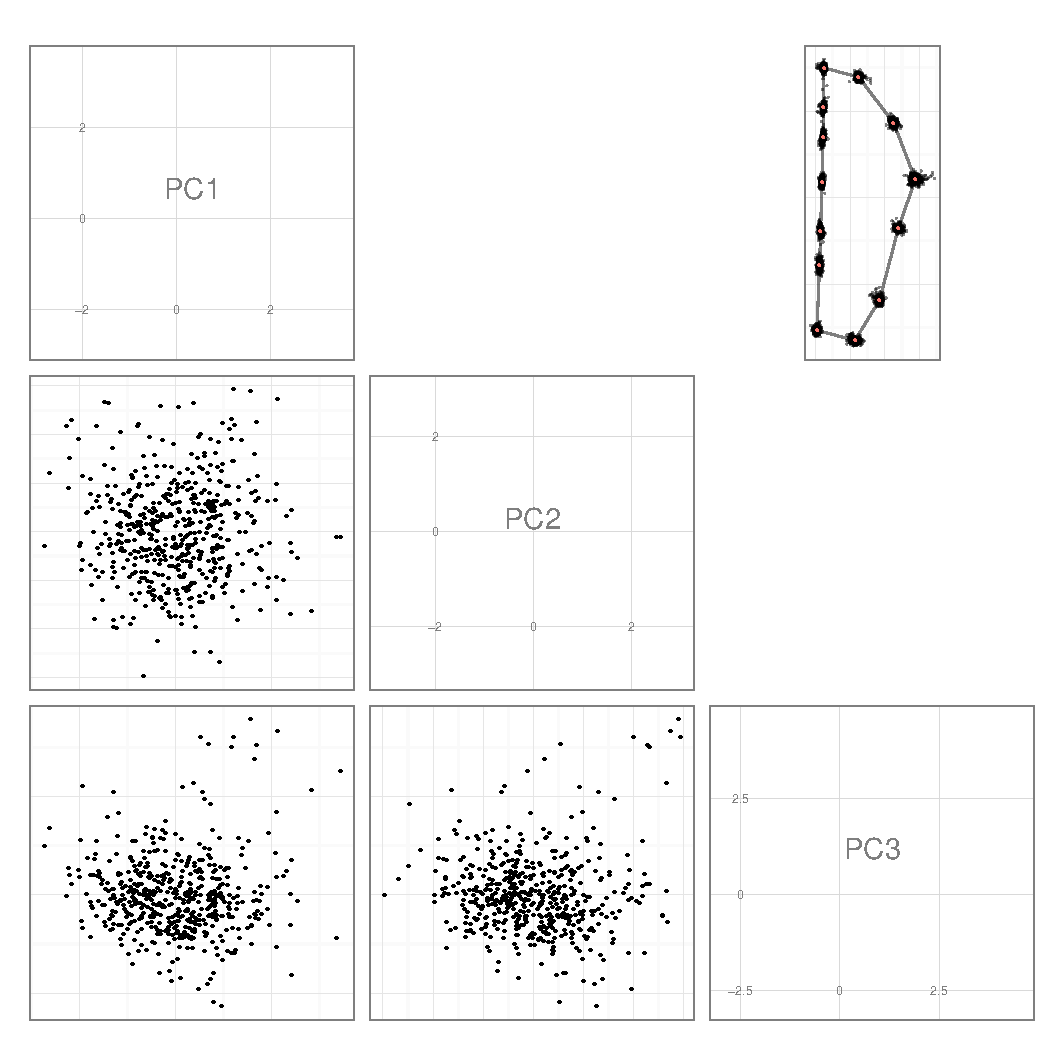
\includegraphics[width = \textwidth]{figure/pca_res}
  \caption{}
  \label{fig:pca}
\end{figure}

\subsection{Machine learning analyses}
\subsubsection{Unsupervised learning}

% PAM results
Comparison of the gap statistic values for the range of PAM solutions indicates that the optimal number of clusters is 1 (Fig. \ref{fig:gap}). The next best clustering solution is two clusters, however there is no geographic structure to this classification scheme, with members of these clusters being seemingly randomly distributed geographically SUPPLEMENT?. Our dataset does not include enough or detailed information on the sex of each \textit{E. marmorata} specimen, thus it is not possible to determine if this clustering solution corresponds to sexual dimorphism between the observations. Male Emyidine turtles are known to have a plastral concavity which may influence landmark position. However, the plastral concavity of \textit{E. mamorata} males is considered less prnounced than in other Emyidine turtles. While we cannot completely rule out sexual dimorphism as the root cause of this observation, we are less concerned with possible effects of sexual dimorphism for the later supervised learning methods.
Increasing the number of clusters does appear to improve the gap statistic enough to merit comparison. 

% figure
%   gap statistic results
\begin{figure}[ht]
  \centering
  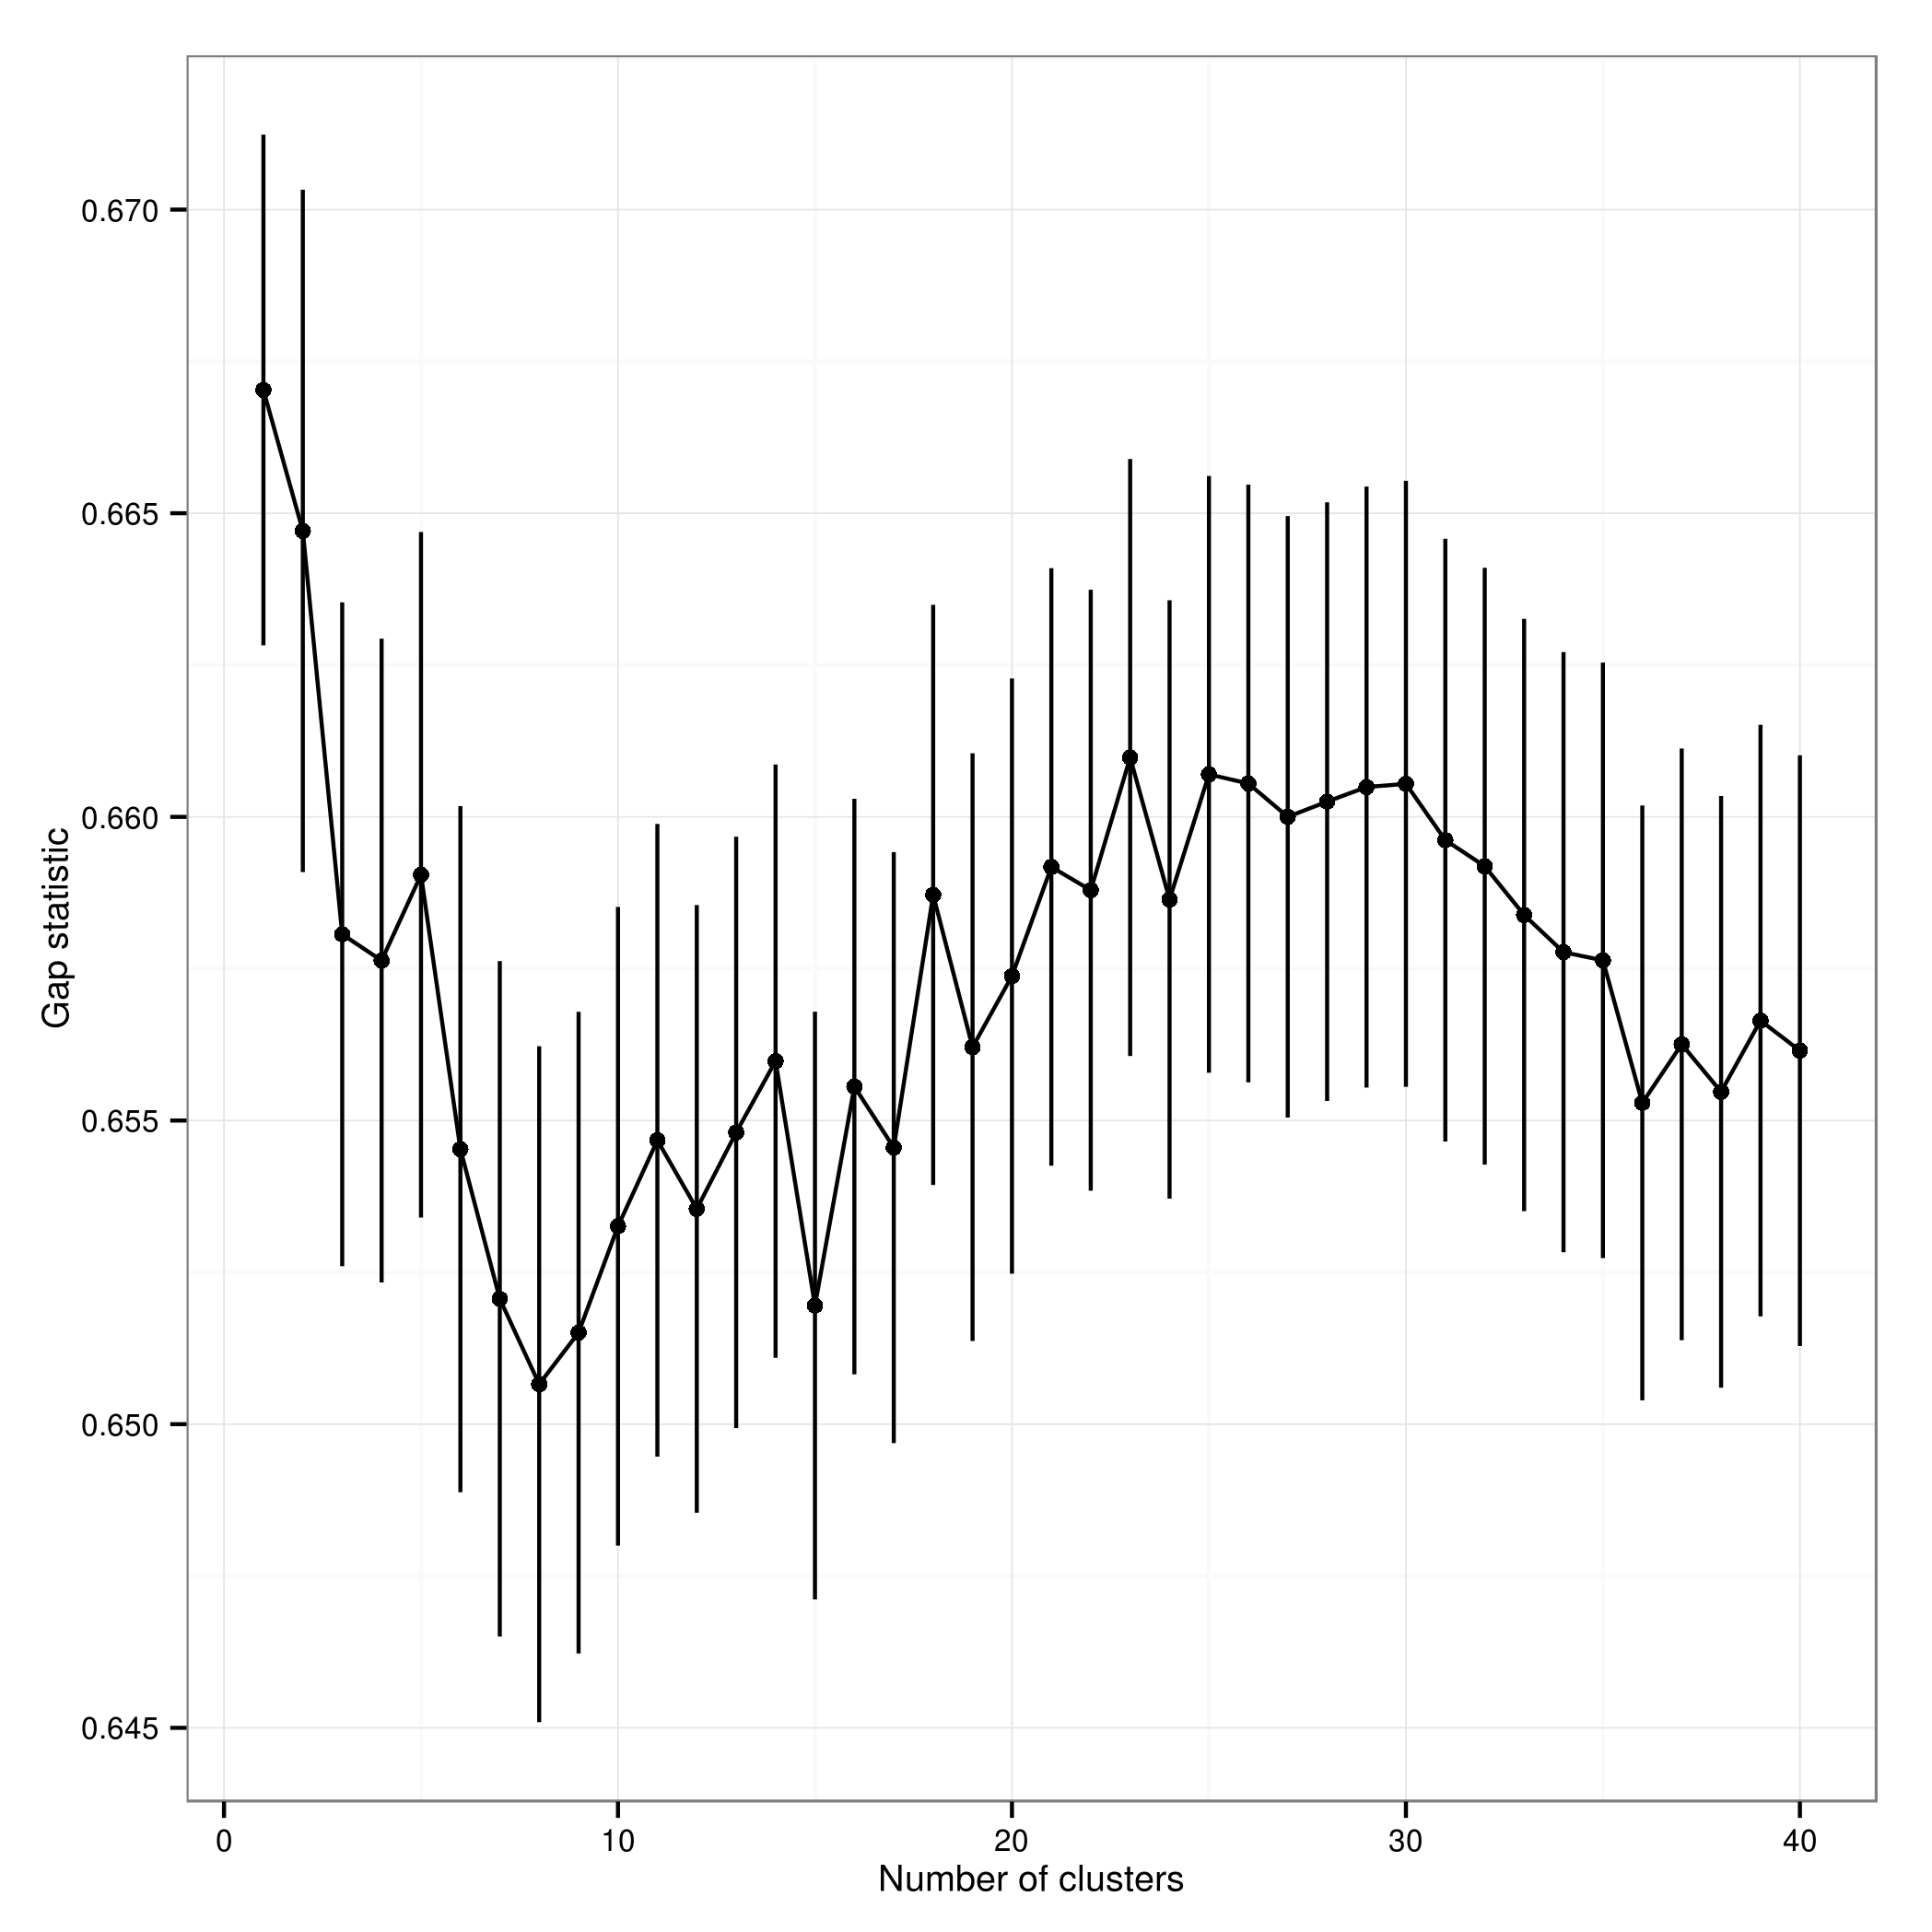
\includegraphics[width = \textwidth]{figure/gap_res}
  \caption{Gap statistic values for PAM clustering results for the \(\rho\) dissimliarity matrix of plastron shape. Error bars are standard errors estimated via 500 bootstrap samples.}
  \label{fig:gap}
\end{figure}

\subsubsection{Supervised learning}
%For all of the classification schemes, the optimal models for both the multinomial logistic regression (Table SUPPLEMENT) and random forest (Fig. \ref{fig:roc}) methods include many, if not most, of the possible features.


% multinomial logistic regression model
The AICc best multinomial logistic regression models, for all four classification schemes, each have the first 10 possible PCs as features (Table SUPPLEMENT). The second best models for all classification schemes had the first 9 PCs as features. The \(\Delta\)AICc values between the optimal and second best model range from 2.0639 for the first morphological based classification hypothesis to 19.8349 for the second molecular based classification hypothesis (Table IN SUPPLEMENT?). The first 10 PCs describe 88.6043874205075\% of total variation in plastral shape.

While the \(\Delta\)AICc value between the optimal and second best model for the first morphological based classification hypothesis was within the range to be considered sufficient and equally optimal \citep{Burnham2002a}, for this analysis we chose to use only the AICc best model. While AICc values can not be compared between models with different responses \citep{Burnham2002a}, we interpret the fact that the optimal model for all classification schemes is the global model as a reason to use the AICc best model for all cases. Additionally, by using a single model for all classification schemes, this limits the number of comparisons between the bootstrap resampled distributions of the AUC values for the testing data set (see below).

% random forest model



The selected number of features in the final random forest model for each classification scheme varied much more than in the case of the multinomial logistic regression models (Fig. \ref{fig:roc}), ranging from 6 for the first morphological based classification hypothesis to 10 for the second morphological based classification hypothesis. 

% need to discuss the final models in both cases.
% figure
%   ROC model selection (see talk)
%   generalize densities
%     facet: multinomial, rf (see talk)

In the case of all models, there is a substantial increase in model performance as measured by AICc for the multinomial logistic models (Tables SUPPLEMENT) or in AUC for the random forest models and illustrated for the multinomial logistic regression models as the number of features increases (Fig. \ref{fig:roc}). 

\begin{figure}[ht]
  \centering
  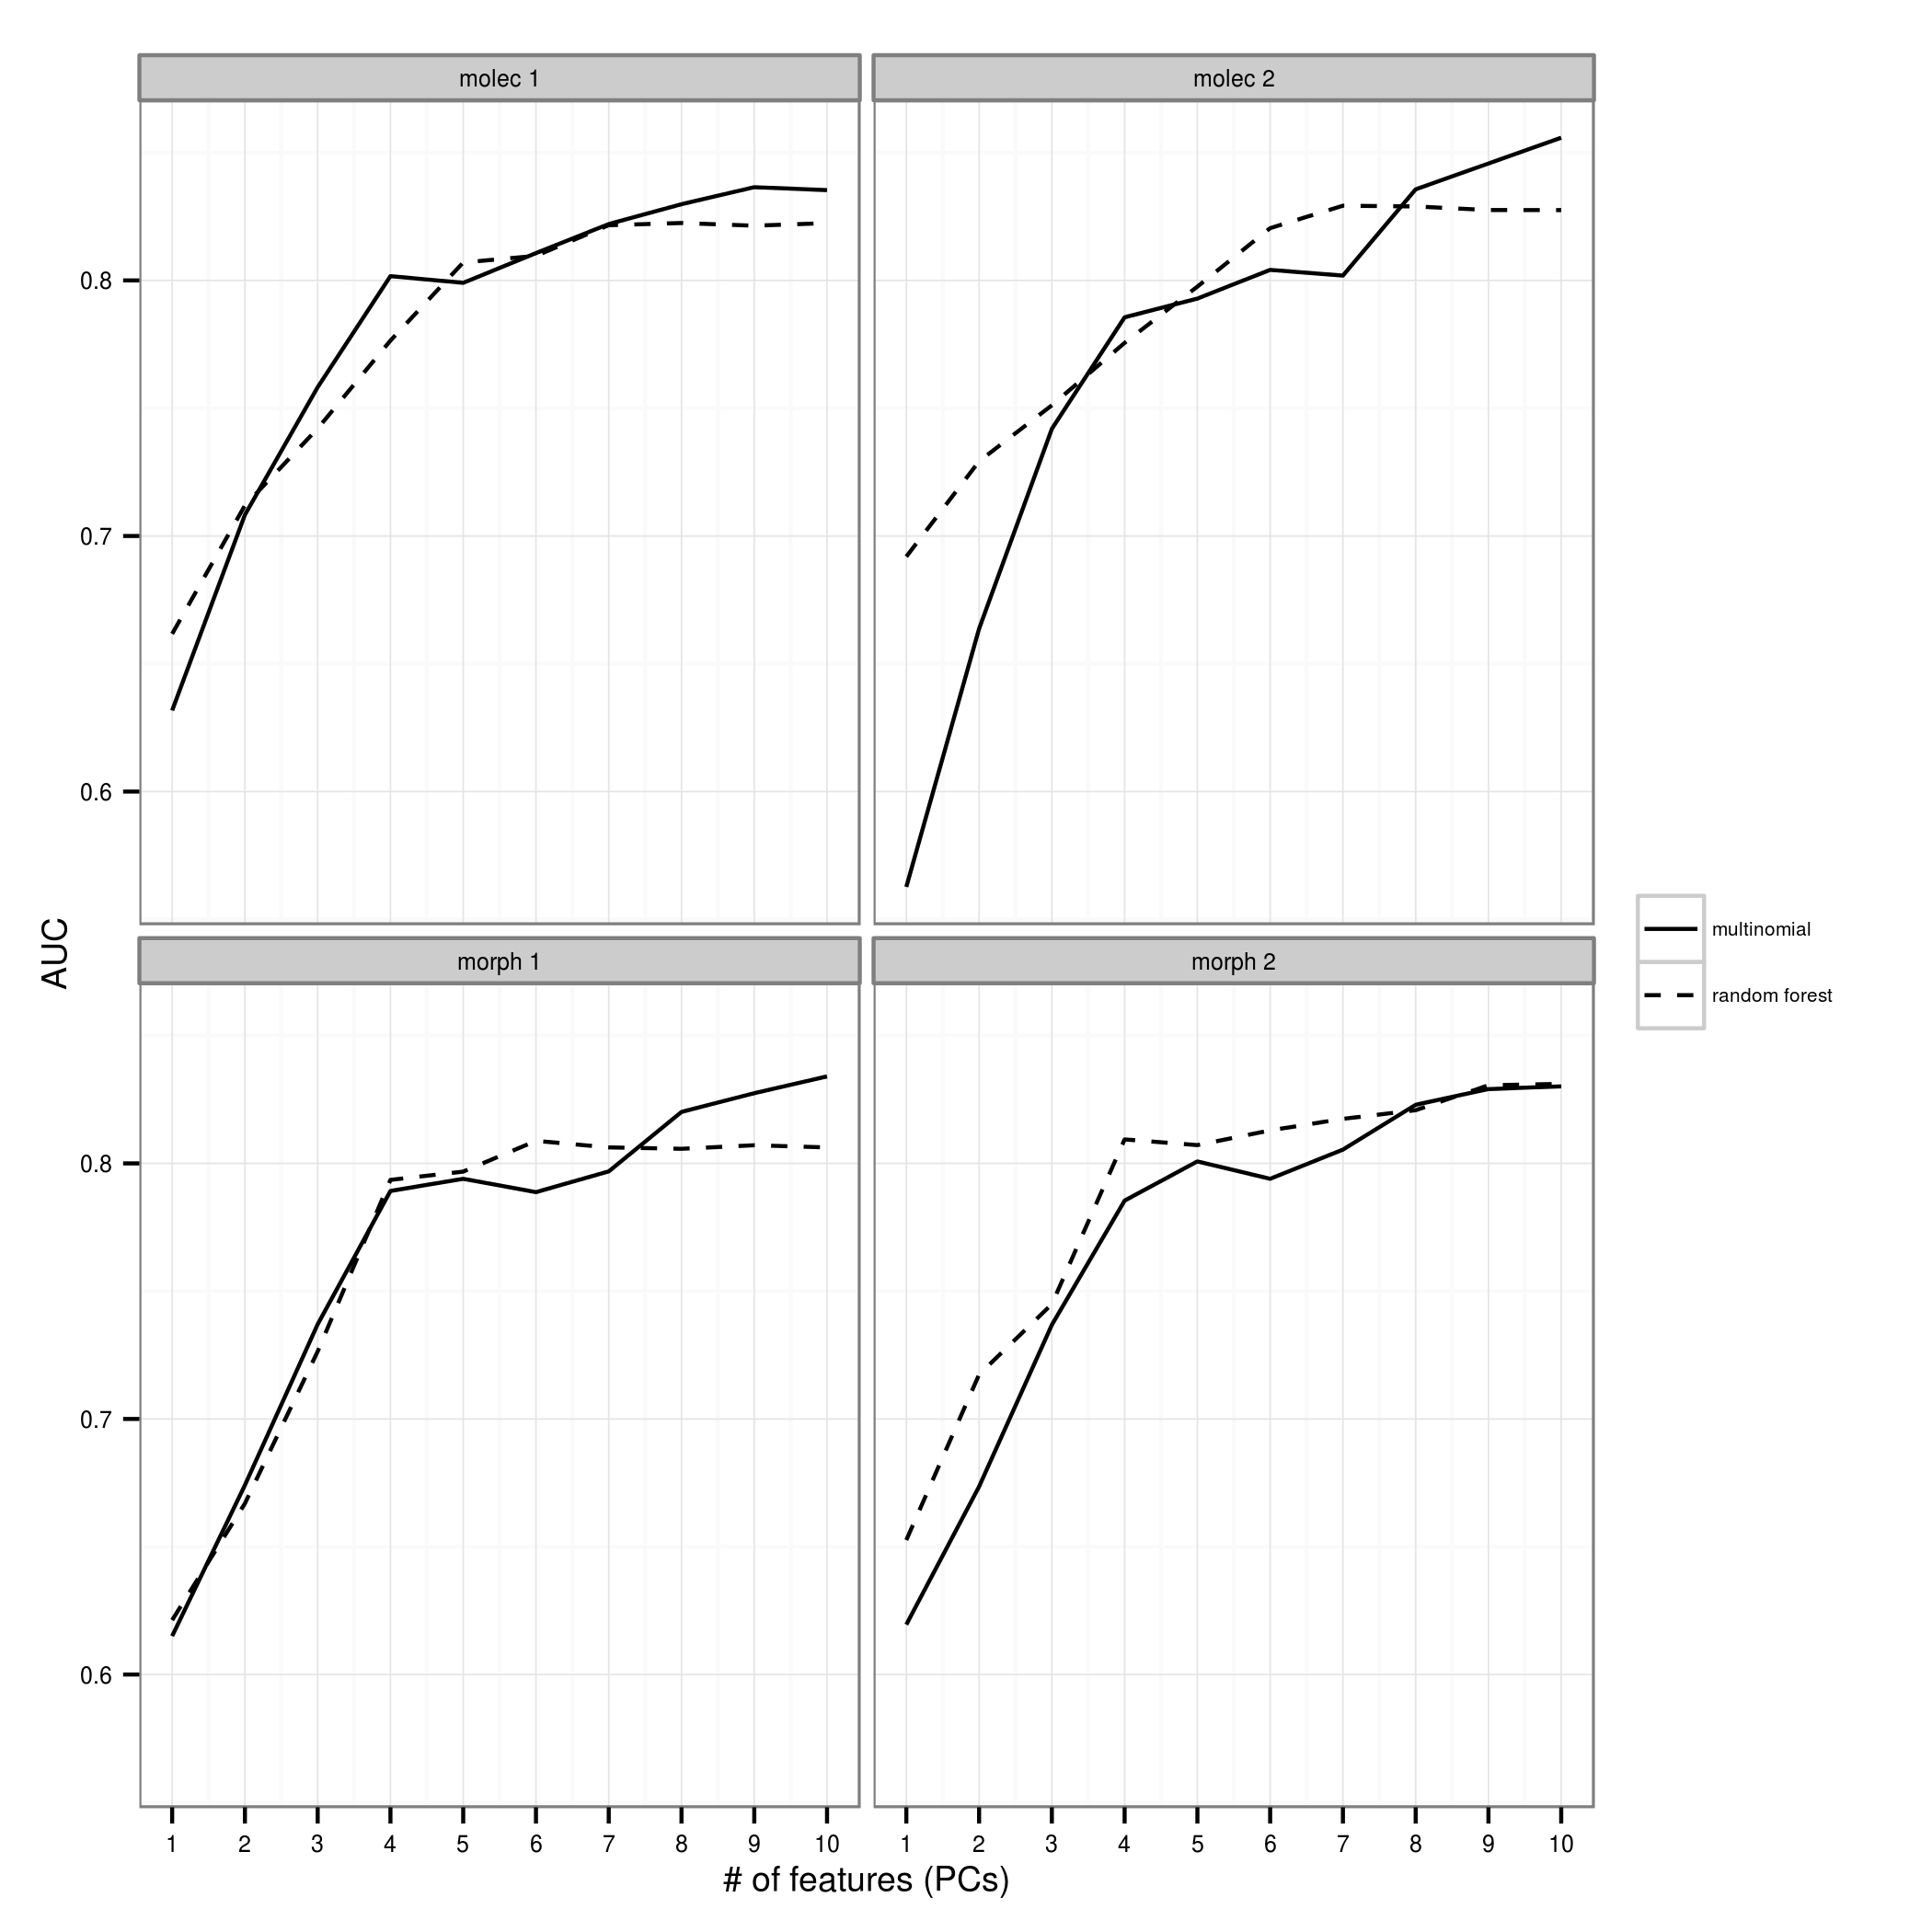
\includegraphics[width = \textwidth]{figure/roc_sel}
  \caption{Effect of increasing the number of PCs as features, or predictors, of classification of plastra for all four classification schemes. As the number of PCs increase, AUC increases until eventually leveling off. Both multinomial logisitic regression and random forest models are illustrated here, though AUC based model selection was only performed for random forest models.}
  \label{fig:roc}
\end{figure}

% table
%   AICc model selection
%   SUPPLEMENT?

%   maps
%     facet: training, multinomial, rf
Results from the generalization of the selected supervised learning models, measured by the distributions of the bootstrapped AUC values of the testing dataset demonstrates that one of the molecular classification hypotheses based on \citet{Spinks2005} and \citet{Spinks2010} was the best overall classification scheme (Fig. \ref{fig:gen_res}). For both methods, the distribution of bootstrapped AUC for the molecular hypothesis was significantly greater MANN-WHITNEY U TEST than all of the other classification scheme. Remarkably, the best classification hypothesis was identical based on both the multinomial logistic regression and random forest models.

\begin{figure}[ht]
  \centering
  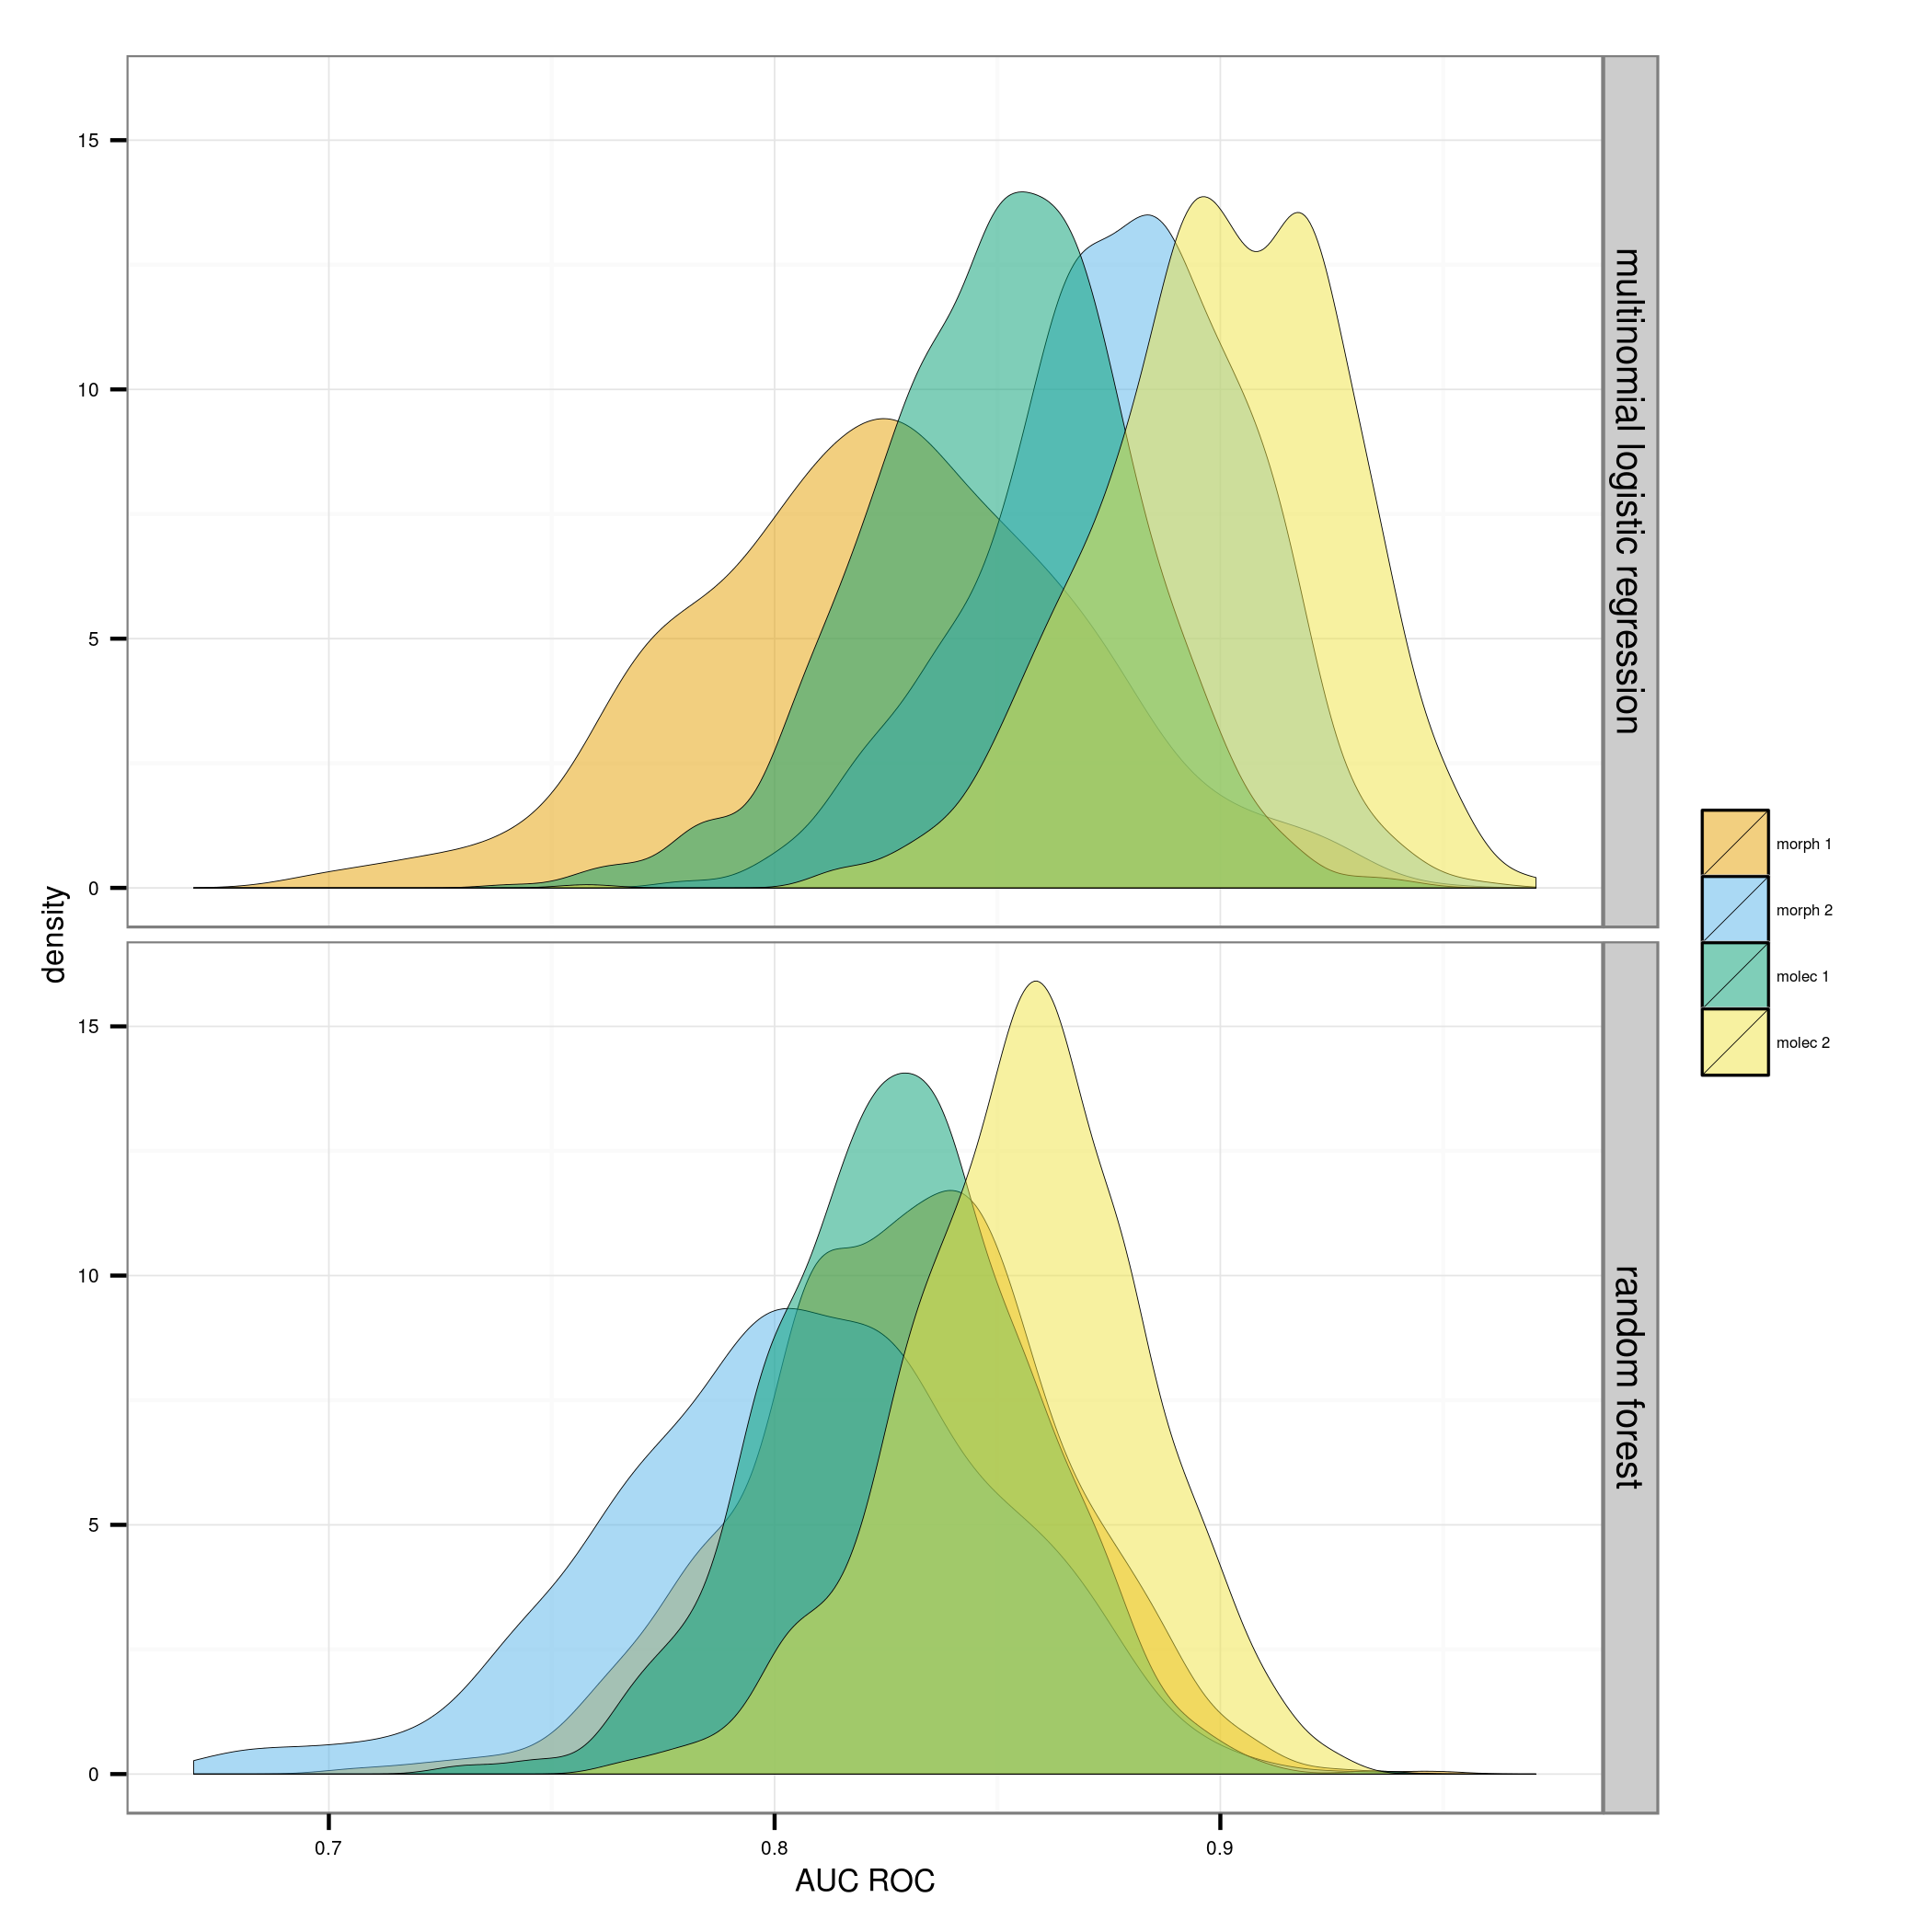
\includegraphics[width = \textwidth]{figure/gen_res}
  \caption{Density estimates of AUC values of predictions of the testing dataset of plastra from 1000 bootstrap resamples. The top facet corresponds to values using the optimal multinomial logistic regression model, as chosen by minimum AICc value. The bottom facet corresponds to the values using the optimal random forest model, as chosen by maximum AUC value.}
  \label{fig:gen_res}
\end{figure}

When the classification results of the training set for the optimal classification scheme are compared with the references classes, the higher AUC value of the best multinomial logistic regression model compared to the best random forest model can be observed as the classifications are much closer to the reference classes (Fig. \ref{fig:gen_map}). The best random forest model misclassified many of the observations as the northern clade instead of the correct class. This systematic misclassification is observable but not as exaggerated in the results of the classifications of the multinomial logistic regression model.

\begin{figure}[ht]
  \centering
  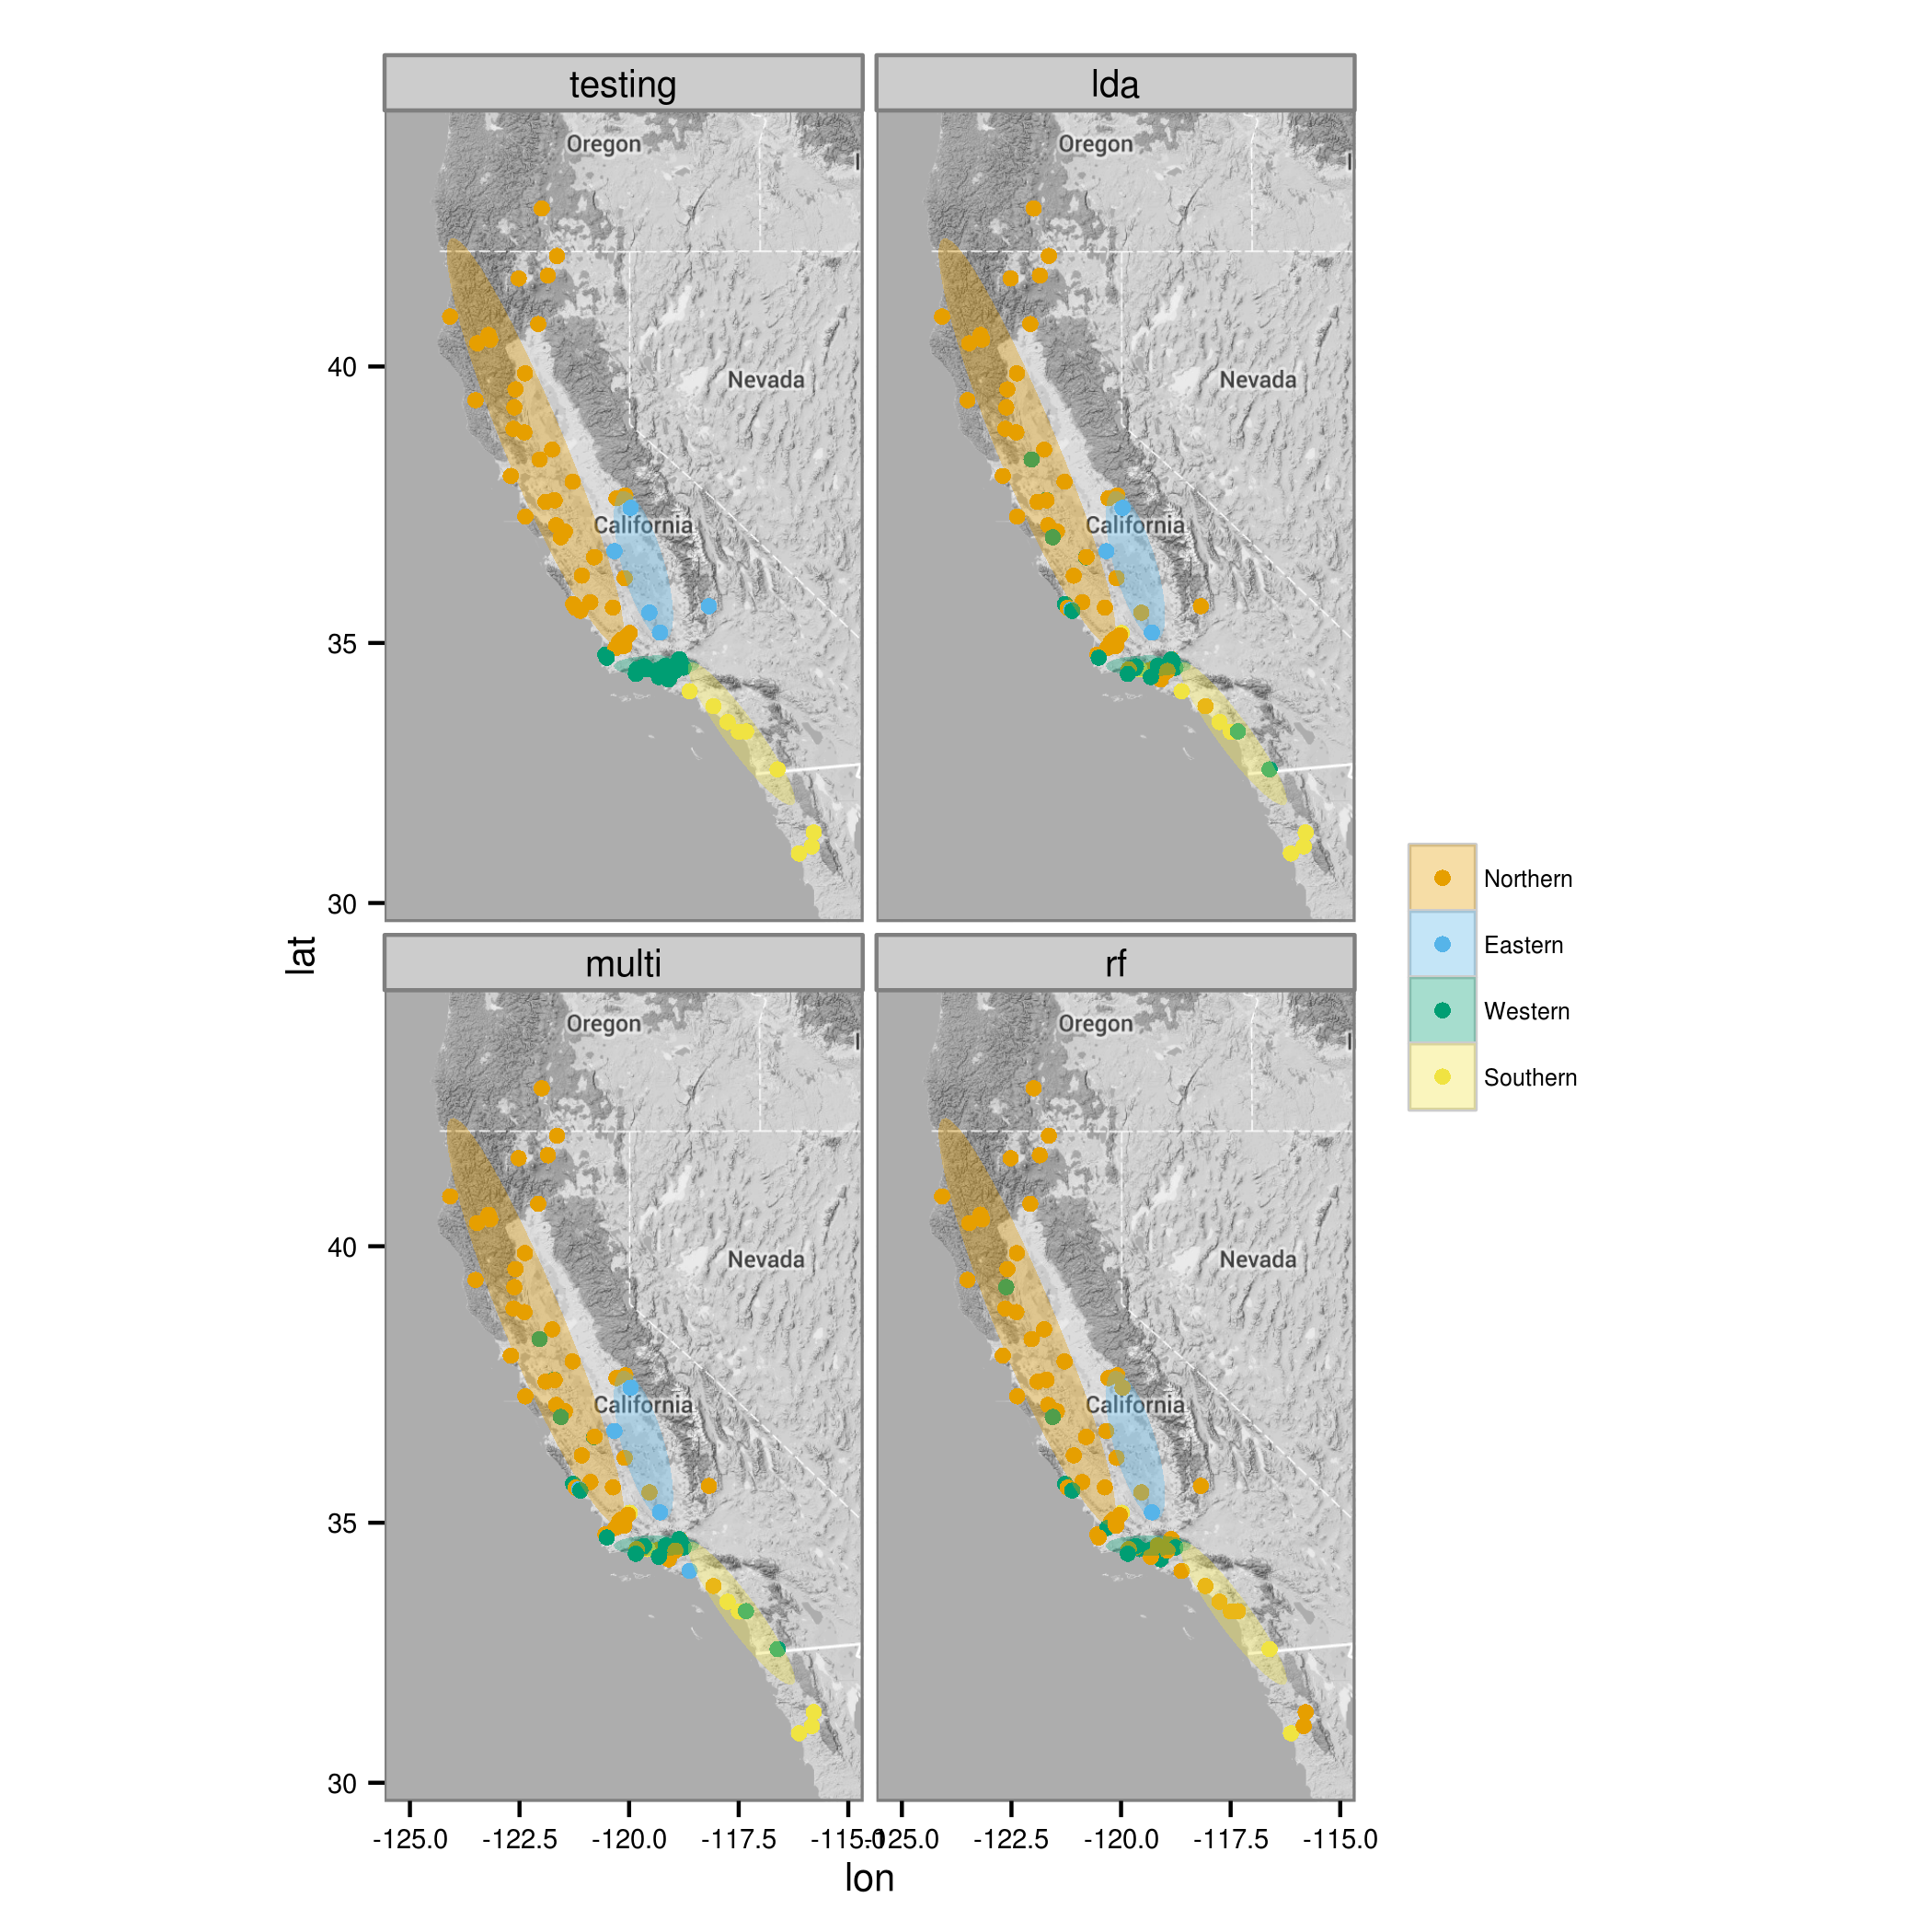
\includegraphics[width = \textwidth]{figure/gen_map}
  \caption{Comparison between reference classification of testing data set and the estimated classifications based on the selected multinomial logistic regression and random forest models, from left to right respectively. Classification corresponds to the four classes as suggested by the hypothesis of \citet{Spinks2005} and \citet{Spinks2010}.}
  \label{fig:gen_map}
\end{figure}

This pattern of misclassification may be caused by the differences in mean shape between each of the different classes (Fig. \ref{fig:mean_shape}). The mean shape of the northern clade is the most similar to the mean shape of the entire dataset (Fig. \ref{fig:mean_shape}, \ref{fig:imp_var}), which may indicate that specimens that are closer to the mean shape will be systematically misclassified as the northern clade.

% mean shapes of all the classes
\begin{figure}[ht]
  \centering
  \begin{subfigure}[b]{0.4\textwidth}
    \centering
    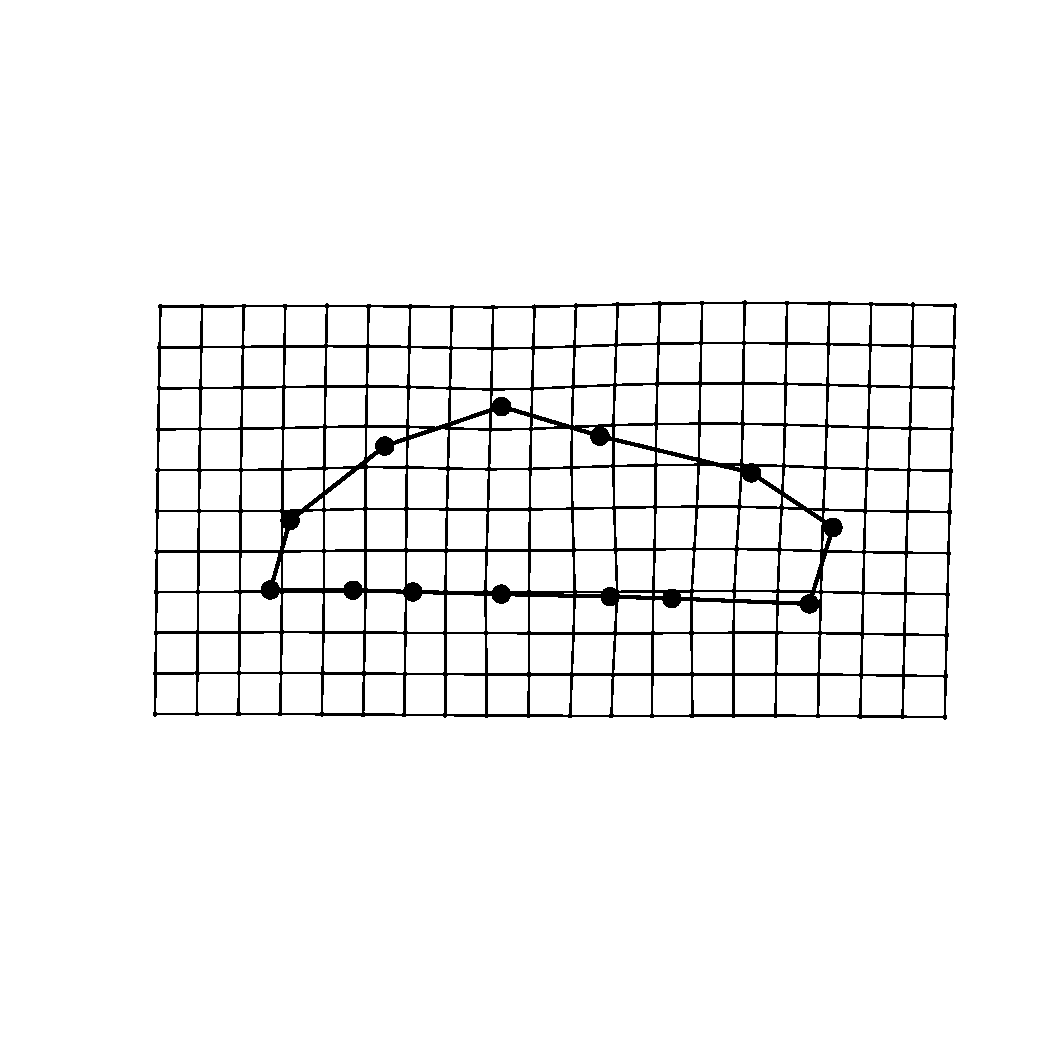
\includegraphics[width = \textwidth]{figure/mshape_1}
    \label{fig:mean_shape1}
  \end{subfigure}
  \begin{subfigure}[b]{0.4\textwidth}
    \centering
    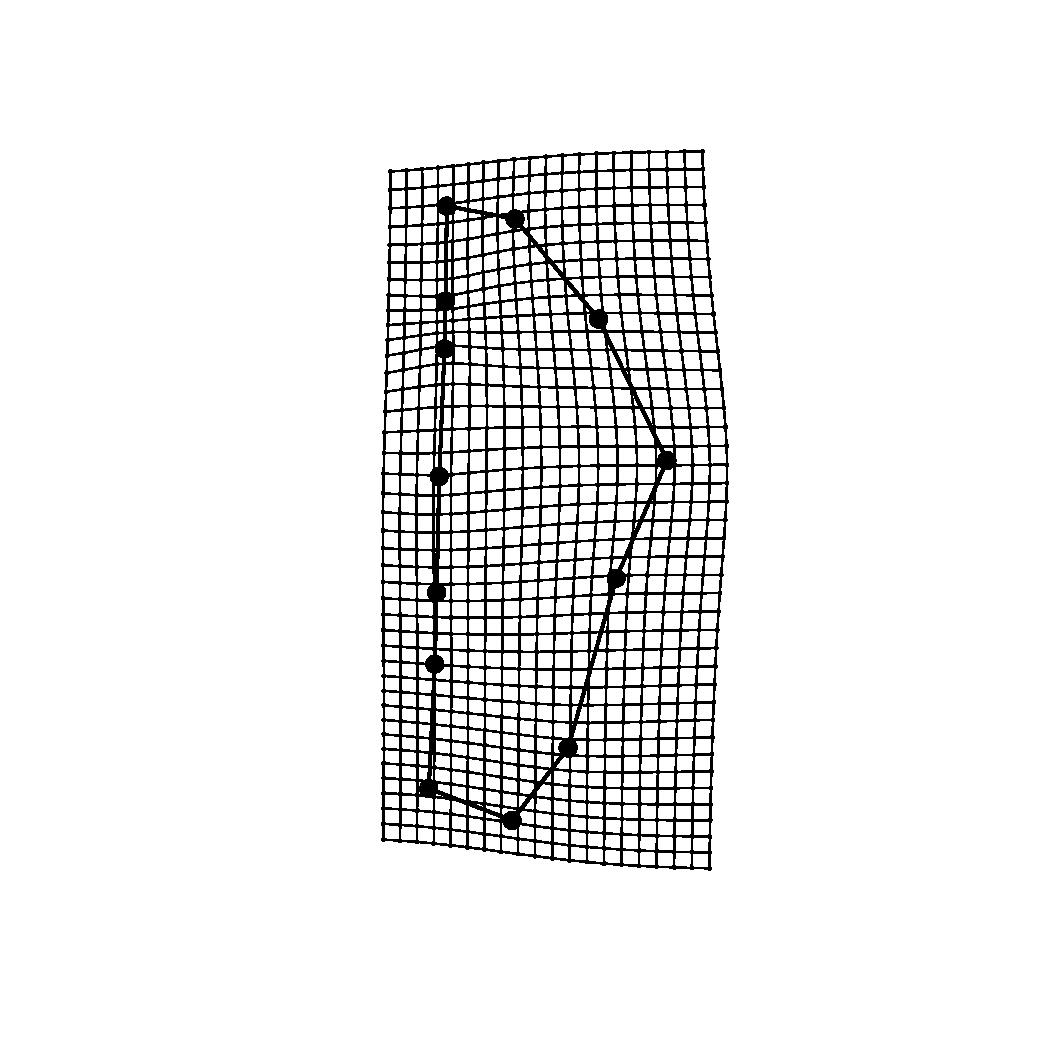
\includegraphics[width = \textwidth]{figure/mshape_2}
    \label{fig:mean_shape2}
  \end{subfigure}
  % new line. might want to make these closer together

  \begin{subfigure}[b]{0.4\textwidth}
    \centering
    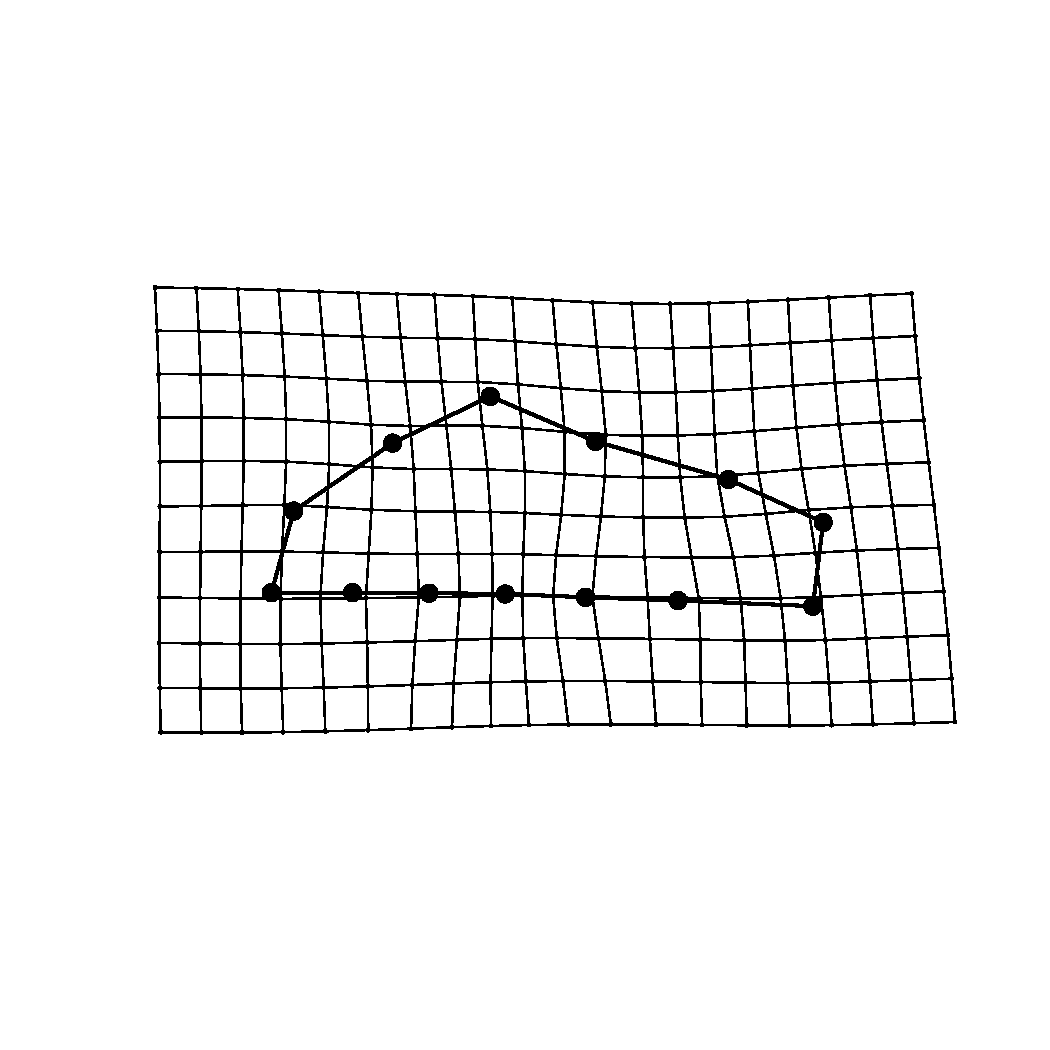
\includegraphics[width = \textwidth]{figure/mshape_3}
    \label{fig:mean_shape3}
  \end{subfigure}
  \begin{subfigure}[b]{0.4\textwidth}
    \centering
    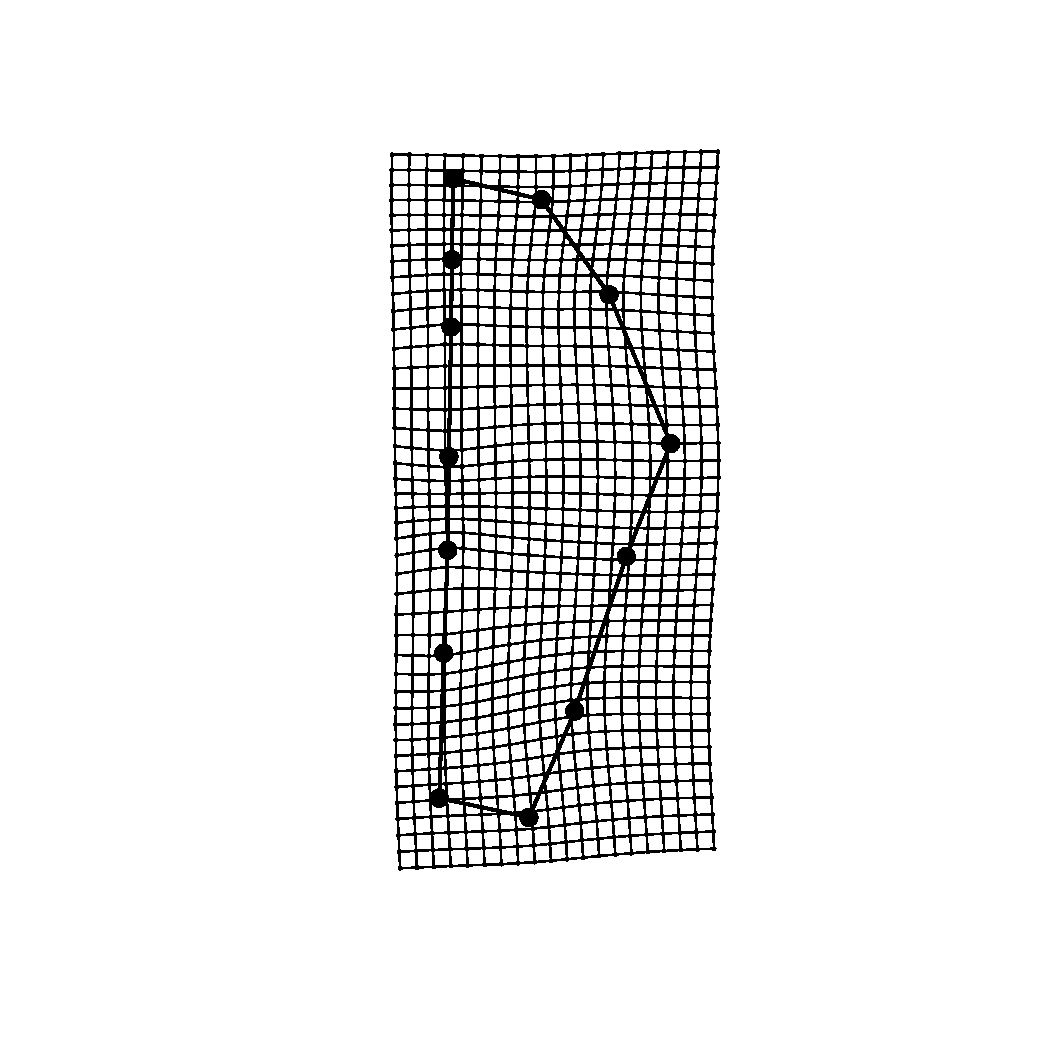
\includegraphics[width = \textwidth]{figure/mshape_4}
    \label{fig:mean_shape4}
  \end{subfigure}
  \caption{2x magnification}
  \label{fig:mean_shape}
\end{figure}

% variation along the most important axes
The results of fitting the final random forest model also include the variable importance for best separating the different classes. The final random forest model of the best classification scheme indicated that after 7 PCs were included as features, AUC would not increase. Of these 7 features, the first three are illustrated here (Fig. \ref{fig:imp_pc}) in descending order of importance SUPPLEMENT WITH VARIABLE IMPORTANCE INFORMATION?. 

\begin{figure}[ht]
  \centering
  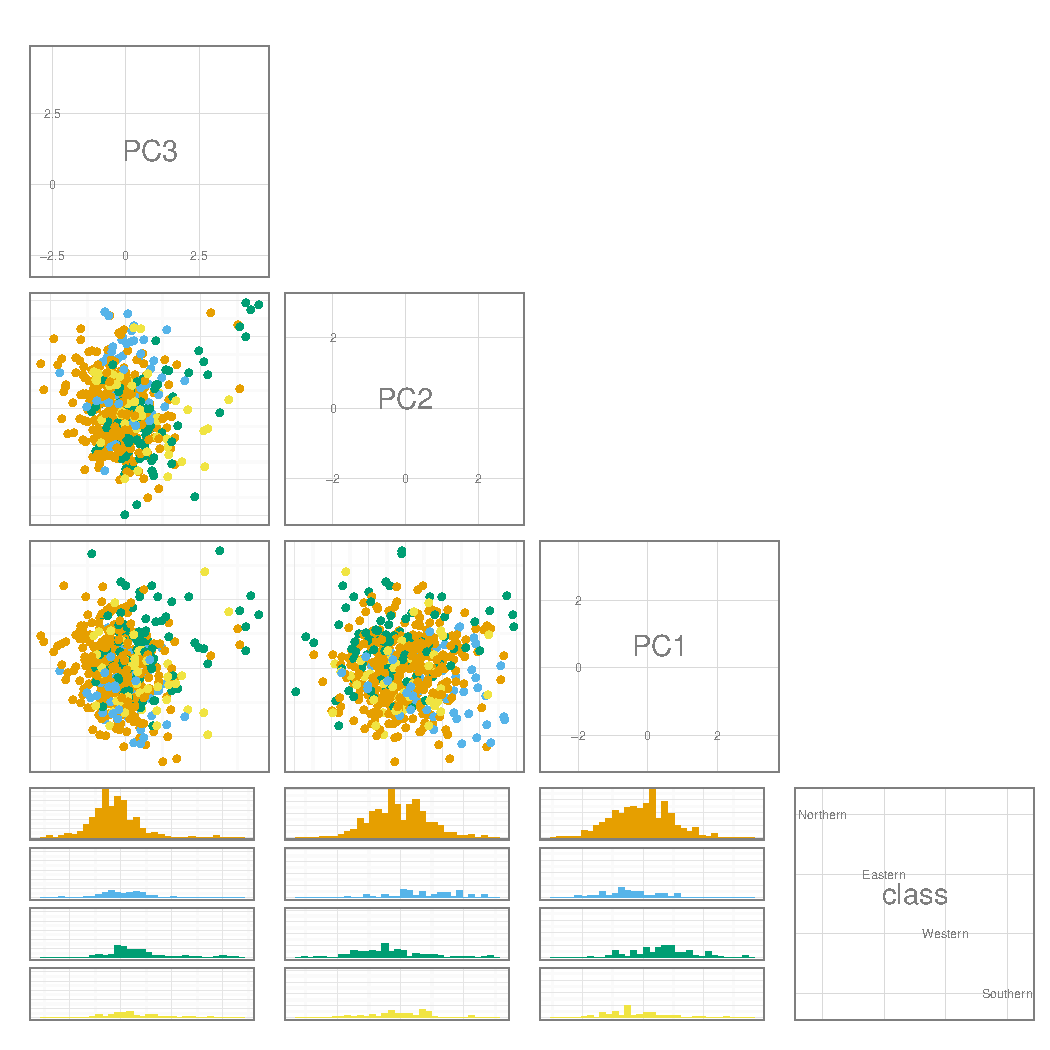
\includegraphics[width = \textwidth]{figure/pca_imp}
  \caption{Pairs plot of the first three most important variables of the optimal random forest model of turtle plastral shape. The variables descend in importance from the upper left to the lower right. The observations are colored as in Figures \ref{fig:gen_res} and \ref{fig:gen_map}.  The bottom row are histograms of classification occurrences along the PCs.}
  \label{fig:imp_pc}
\end{figure}
% need to add in variance percentages on the different axes.

The first two most important features describe different aspects of variation (Fig. \ref{fig:imp_var}). The third PC, or first most important PC, describes variation in the relative position of landmarks on anterior and posterior portions of the plastron and represents 9.6697\% of total variation. The eighth PC, or second most important PC, mostly describes variation in landmarks along the midline of the plastron and represents 4.1061\% of total variation. The major variations along these axes correspond well to the differences between the class means and the mean plastron shape (Fig. \ref{fig:mean_shape}) where major class differences seem based on the relative ballooning or shrinking of the anterior and posterior portions of the plastron together.

\begin{figure}[ht]
  \centering
  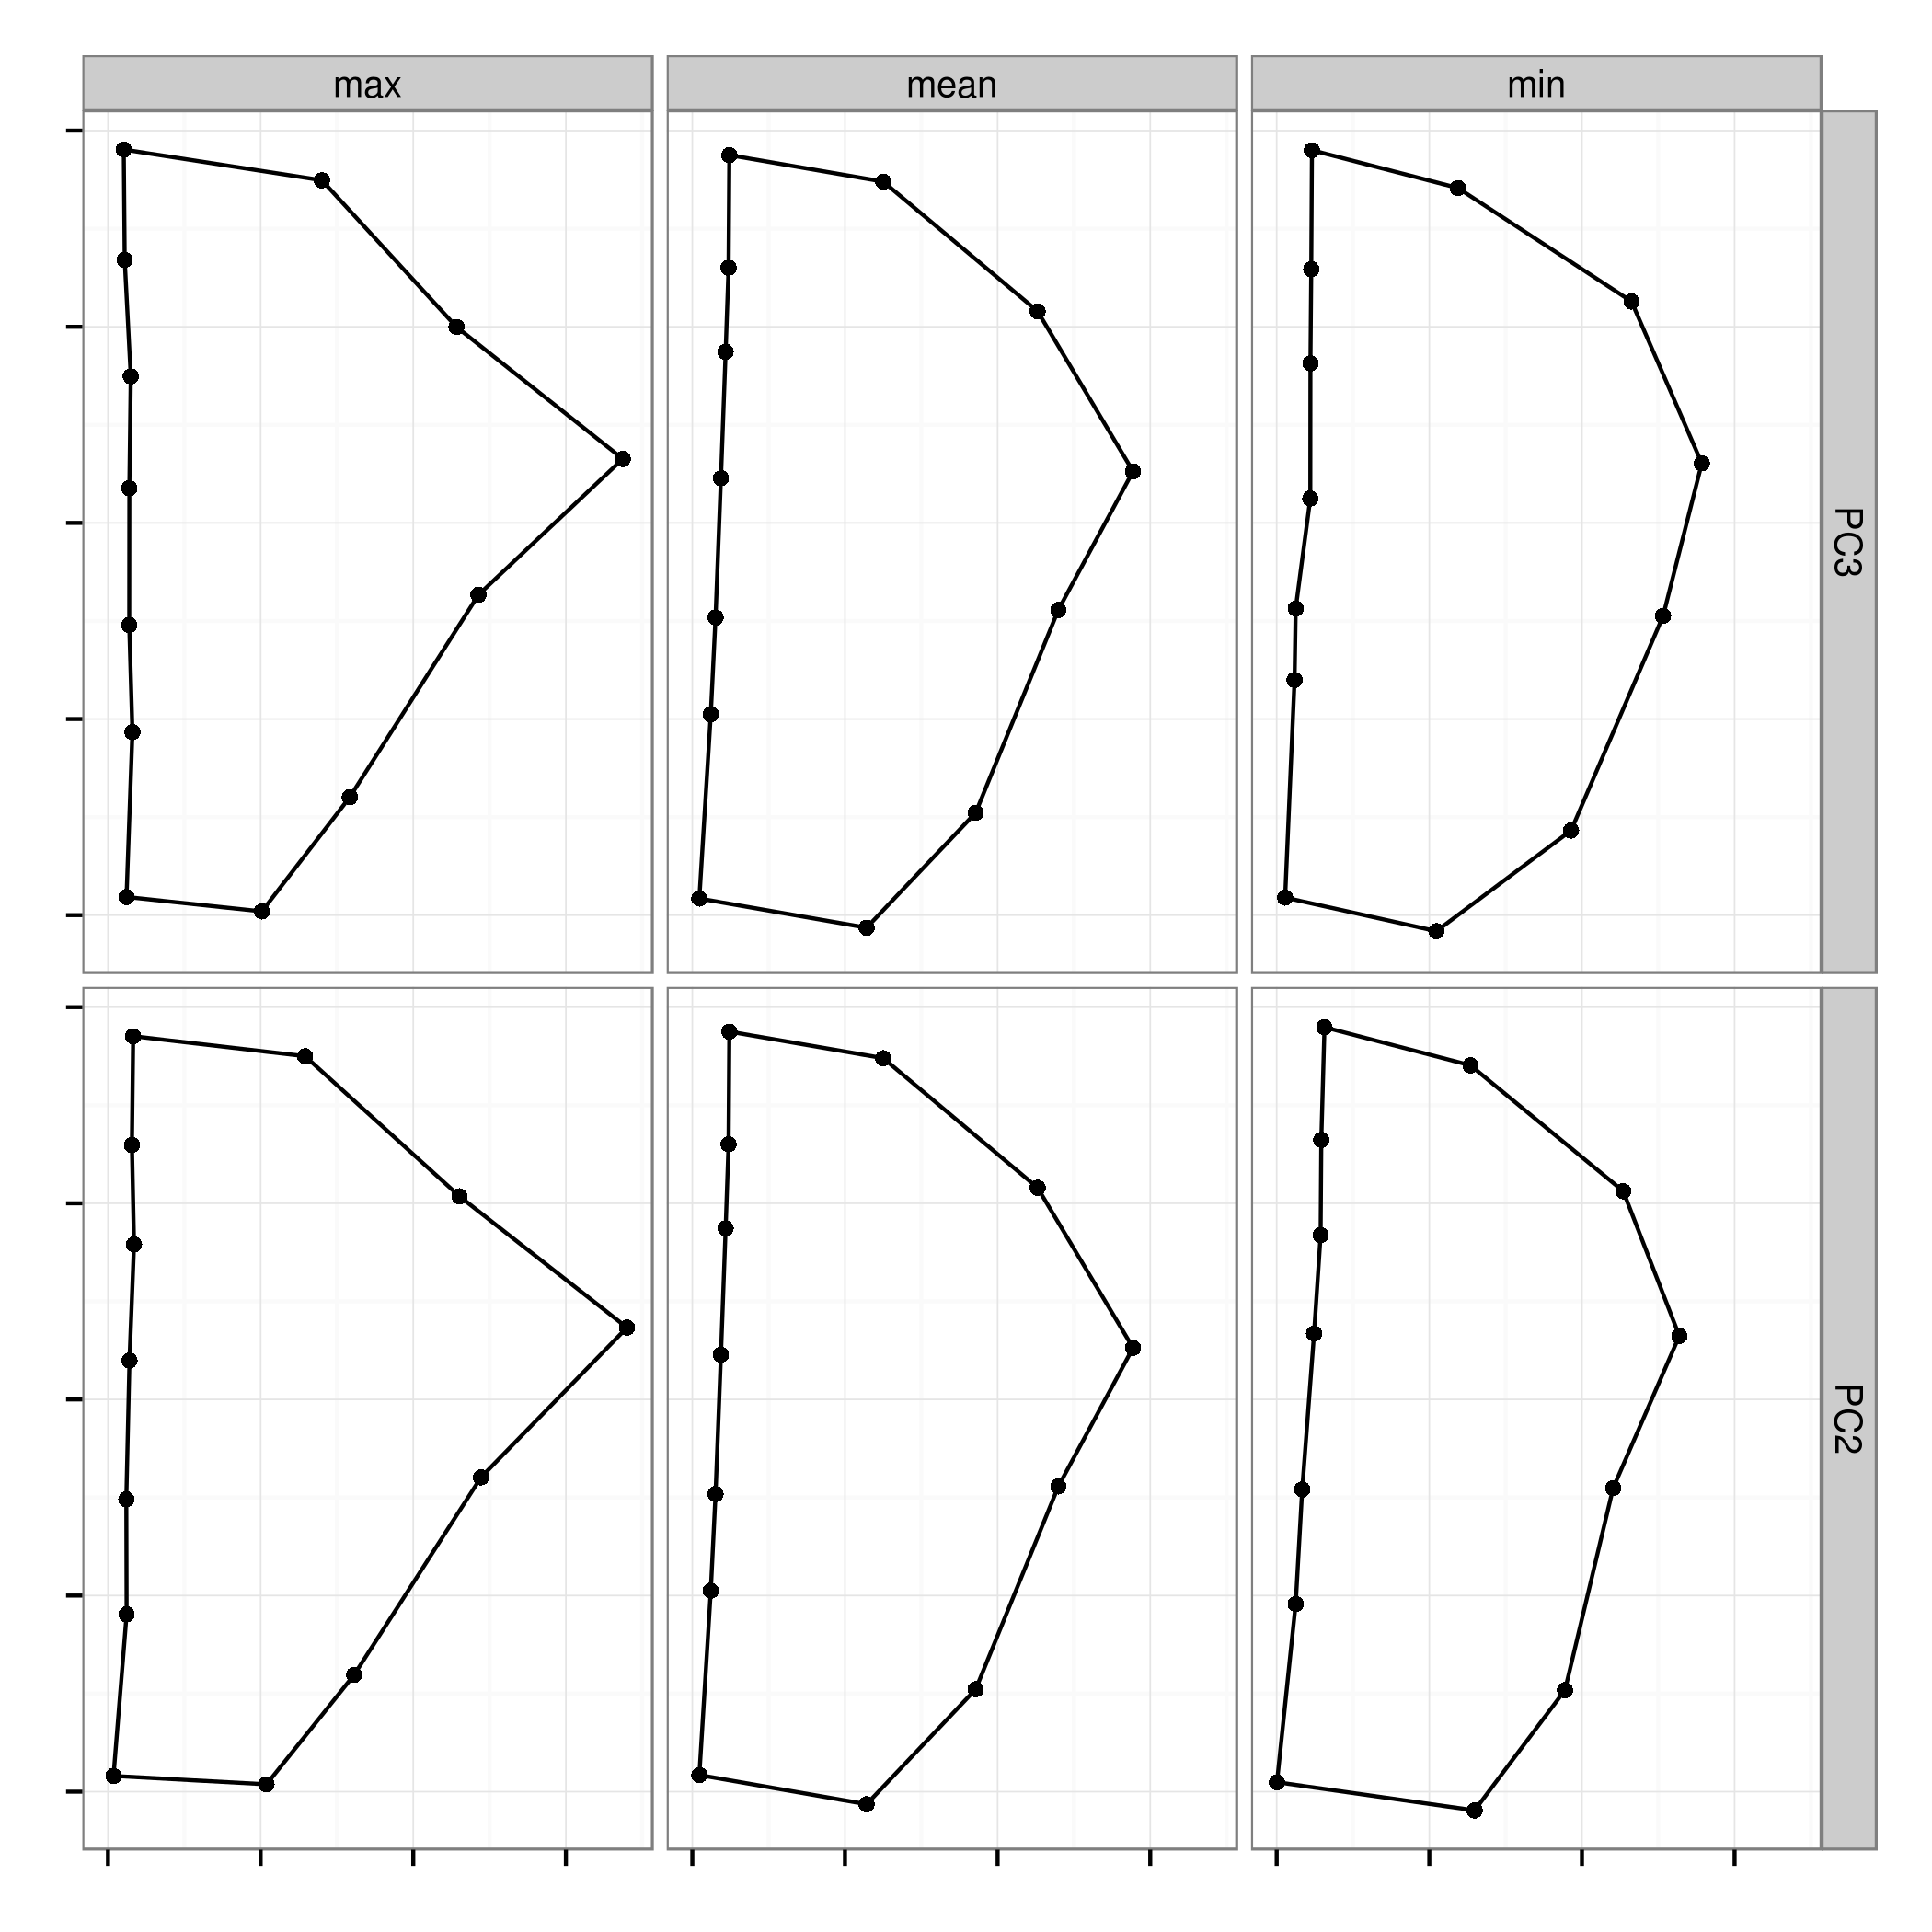
\includegraphics[width = \textwidth]{figure/imp_var}
  \caption{Landmark variation along the two most important features (PCs) based on the final random forest model. The first row corresponds to the third PC and the second corresponds to eighth PC. Landmark configurations are minimum observed on that PC, mean shape, and maximum observed on that PC.}
  \label{fig:imp_var}
\end{figure}

\section{Discussion}
% discussion of results
%   remarkable concordance in the supervised learning methods
The results of this study provide support for the mitochrondial based hypothesis of classification of \textit{E. marmorata} \citep{Spinks2005,Spinks2010}. This is contrary to the original classification of \textit{E. marmorata} \citep{Seeliger1945} and lends credence to the idea that at least some aspect of cryptic diversity is a product of sample size, methodology, or both.

%   what does this mean about cryptic diversity?
%   unsupervised learning shortcomings

The lack of coherent geographical subclass assignment from PAM clustering (Fig. \ref{fig:gap}) as well as the large number of features necessary before no increase in AUC for all models (Fig. \ref{fig:roc}) indicates that the morphological variation between subclasses is extremely fine grained. This was also exemplified by the small differences in mean class shape for the final chosen classification scheme (Fig. \ref{fig:imp_var}).

% methodological concerns
%   compromise in the supervised learning models
%     fair because as much variation as ``necessary'' is used
The methods presented here for supervised learning analysis of the landmark variation represent a compromise between explicitly modeling all shape variation and preventing models from being overfit and ungeneralizable. While all aspects of shape may be evolving simultaneously, and not along individual PCs, including all PCs as predictors in each model might increase model complexity beyond a reasonable level for the sample size or the necessary complexity to accurately model the response. However, this compromise is not without its advantages. Because the AICc and AUC values improved rapidly with increased model complexity (Fig. \ref{fig:roc}),k this indicated how fine scale the actual variation between classes was and how necessary including many PCs was. Additionally, the relative risk values from the mulitinomial logistic regression models demonstrate MORE STUFF HERE. Also, the systematic misclassification of the final random forest model and the possible relationship with the similarity the mean shape of the northern clade and the overall mean shape (Fig. \ref{fig:gen_map}, \ref{fig:mean_shape}) is a good indicator of the very fine scale variation between classes.

%   unsupervised learning
%     model based clustering
%     nonparametric bayesian approach
%     anything about semisupervised clustering? probably not
Ultimately, it would be most useful to not require such explicit classification hypotheses, especially when concerned about possible cryptic variation in extinct taxa. The only unsupervised method employed in this study, PAM, is rather simple and not model based. Comparison here was facilitated via a summary statistic and bootstrapped confidence intervals. A more useful approach would be employing various model based clustering approaches CITATIONS. In this manner, a series of candidate models can be compared via model comparison methods, such as AIC or Bayes factors CITATION, in order to asses the best clustering solution.% Of particular note are nonparametric Bayesian approaches to model based clustering CITATIONS. This approach uses a class of flexible priors to allow for the most optimal clustering solution to be decided from the data. Currently, there exists a nonparametric Bayesian clustering method and further development of this approach may prove extremely fruitful for better delimiting taxa solely from morphology.

% future directions
%   conservation utility
%   fossil diversity
%     current approach favors having an extremely explicit classification hypothesis
%     as indicated about, nonparametric bayes and other model based clustering can help

% closing statements
In this study we have demonstrated that given a large sample size and alternative methodology, it is possible to determine which classification scheme best explains variation in a taxon amongst a set of alternative hypotheses. The observed plastral variation of \textit{E. marmorata} is most consistent with the mitochondrial based hypothesis of \citet{Spinks2005} and \citet{Spinks2010} and not with the original morphology based hypothesis of \citet{Seeliger1945}. We have also demonstrated the utility of various machine learning approaches to understanding variation in morphometric data. Specifically, better understanding odds misclassification and identifying which is the most important for delimiting different classes. These methods represent new applications which may be important for future studies interested in class-based morphological comparison and variation, both in the context of cryptic diversity and with known classifications.

\section{Acknowledgements}
PDS would like to thank David Bapst, Michael Foote, Benjamin Frable, and Dallas Krentzel for useful discussion which enhanced the quality of this study.

\bibliographystyle{sysbio}
\bibliography{turtle,packages}

\end{document}
